
\documentclass[master]{kuisthesis}		% 修士論文(和文)

%\usepackage[dvipdfmx]{graphicx}
\usepackage[draft]{graphicx}
\usepackage{latexsym}
\usepackage[fleqn]{amsmath}
\usepackage[psamsfonts]{amssymb}
\usepackage{bm}
\usepackage{txfonts}
\usepackage{booktabs}
\usepackage[dvipdfmx]{color}
\usepackage{comment}
\usepackage{epsfig}
\usepackage{subfig}

\makeatletter

\newcommand{\argmax}{\mathop{\rm arg~max}\limits}
\newcommand{\argmin}{\mathop{\rm arg~min}\limits}
\newcommand{\sij}{(i,j)}
\newcommand{\mN}{{\mathcal N}}
\newcommand{\pij}{p^{(i,j)}}
\newcommand{\rd}{r^{\sij}_{\rm d}}
\newcommand{\ru}{r^{\sij}_{\rm u}}
\newcommand{\rij}{r^{\sij}}
\newcommand{\etau}{\eta_{\rm u}^{(j)}}
\def\coloneqq{\mathrel{\mathop:}=}
\newcommand{\sijk}{(i,j,k)}
\newcommand{\pijk}{p^{(i,j,k)}}
\newcommand{\rijk}{r^{(i,j,k)}}
\newcommand{\mthc}{\mathcal C}
\newcommand{\mthni}{{\mathcal N}_i}
\newcommand{\mthnj}{{\mathcal N}_j}
\newcommand{\mthnk}{{\mathcal N}_k}

%\newcommand{\pic}[5]{
%	\begin{figure}[#1]
%		\centering
%		\ifnum \figtab=1
%			\includegraphics[width=#2\textwidth]{#3}
%		\fi
%		\caption{#4\label{#5}}
%	\end{figure}
%}
%	(例)
%	\pic{!t}{0.6}{./fig/C_H_matome.eps}{Area-coverage hole $|\mathcal{H}(\bm{p})|$}{fig:ch3}

%----------- マクロ ----------
%数式番号を節毎に分けてリセットする
\begin{comment}
\def\theequation{\arabic{section}.\arabic{equation}}
  \makeatletter
  \@addtoreset{equation}{section}
  \makeatother
%図番号を節毎に分けてリセットする
\makeatletter
 \renewcommand{\thefigure}{%
   \arabic{section}.\arabic{figure}}
  \@addtoreset{figure}{section}
\makeatother
%表番号を節毎に分けてリセットする
\makeatletter
 \renewcommand{\thetable}{%
   \arabic{section}.\arabic{table}}
  \@addtoreset{table}{section}
\makeatother


\def\LATEX{{\rm (L\kern-.36em\raise.3ex\hbox{\sc a})\TeX}}
\def\LATex{\iLATEX\small}
\def\iLATEX#1{L\kern-.36em\raise.3ex\hbox{#1\bf A}\kern-.15em
    T\kern-.1667em\lower.7ex\hbox{E}\kern-.125emX}
\def\LATEXe{\ifx\LaTeXe\undefined \LaTeX 2e\else\LaTeXe\fi}
\def\LATExe{\ifx\LaTeXe\undefined \iLATEX\scriptsize 2e\else\LaTeXe\fi}
\let\EM\bf
\def\|{|}
\def\<{\(\langle\)}
\def\>{\(\rangle\)}
\def\CS#1{{\tt\string#1}}
\end{comment}

\setcounter{topnumber}{5}%    ページ上部の図表は 5 個まで
\def\topfraction{1.00}%       ページの上 1.00 まで図表で占めて可
\setcounter{bottomnumber}{5}% ページ下部の図表は 5 個まで
\def\bottomfraction{1.00}%    ページの下 1.00 まで図表で占めて可
\setcounter{totalnumber}{10}% ページあたりの図表は 10 個まで
\def\textfraction{0.04}%      ページうち本文が占める割合の下限
%        これを 0 にすると本文が 1 行だけのページが出来る
%        0.04 くらいにすると 1 行だけのページは防げる
%        0.1 くらいが良いかも知れない
\def\floatpagefraction{0.7}%  図表だけのページは少なくとも
                          %  これだけを図表が占める

\jtitle[全二重通信無線LANにおけるメディアアクセス制御]%	% 和文題目(内容梗概/目次用)
	{全二重通信無線LANにおけるメディアアクセス制御}	% 和文題目
\etitle{\normalsize Media Access Control for In-Band Full-Duplex wireless LANs}	% 英文題目
\jauthor{飯田 直人}				% 和文著者名
\eauthor{Naoto IIDA}			% 英文著者名
\supervisor{守倉 正博 教授}			% 指導教員名
\date{平成28年2月8日}				% 提出年月日
\department{通信情報システム}				% 修士論文の場合の専攻名

\begin{document}
\maketitle					% 「とびら」の出力

\begin{jabstract}				% 和文梗概
	無線LAN(Local Area Network)システム大容量化を実現する方法の一つとして,送受信を同時に同一帯域で行うの全二重通信が有望である.
	全二重通信無線LANにおいては,同時に送信される二つのデータフレームの時間長が異なる場合にチャネルが空いた無駄時間が生じ,
	スループットが低下するという問題がある.
	更に,下り通信を受信するSTAとAPへ上り通信を行うSTAが異なるUFD(user-multiplexing Unidirectional Full-Duplex)通信においては,
	APへ上り通信を行うSTAの送信信号がAPからの下り通信に干渉を与えるユーザ間干渉によってスループットが低下するという問題がある.
	それに対し,ユーザ間干渉が少なくなるようなSTA組を選択しスループットを最大化する手法の提案がなされているが,
	STA間の不公平性やSTAの遅延時間の増大といった課題が残されている.
	\par
	本論文では,この2つの問題に対して解決を図る.
	まず,前者のフレーム時間長の違いによる無駄時間の発生に対しては,フレーム時間長最適化手法を提案する.
	フレームアグリゲーション技術を用いて,同時に送信される二つのデータフレームの内,
	一方のフレームの時間長を最適化問題を解くことで他方のフレームの時間長に揃え,無駄時間を削減する.
	計算機シミュレーションにより,提案手法が無駄時間を削減し,スループットを向上させることを示す.
	次に,後者のUFD通信に関する問題に対しては,公平性を改善するための送受信STA選択手法を提案する.
	提案手法では,STA間の公平性を考慮したSTA選択を最適化問題として定式化し,各STA組によって通信が行われる確率を求める.
	得られた確率をもとに送受信を行う2台のSTAを確率的に決定する.
	さらに,遅延時間を削減するためにUFD通信加え,上りOFDMA(Orthogonal Frequency Division Multiple Access)を用いるためのSTA選択手法を提案する.
	OFDMAによって上り通信を多重化することでSTAの送信機会を増加させ,遅延時間を削減する.
	計算機シミュレーションにより,提案手法が公平性の改善とスループットとのトレードオフの調整,遅延時間の削減が実現されることを示す.
\end{jabstract}

\begin{eabstract}				% 英文梗概
	An in-band full-duplex system is one of the solutions for improving the throughput performance of wireless local area networks (WLANs), which allows nodes to transmit and receive simultaneously in the same frequency band. In in-band full-duplex WLANs, the difference of time length of data frames transmitted by an AP and an STA wastes the frequency channel and decreases the throughput performance. Moreover, in the user-multiplexing unidirectional full-duplex (UFD) communication, inter-user interference decrease the throughput performance. To mitigate the inter-user interference, STA-pair selection schemes have been discussed.
	However, since these schemes select pairs of STAs so that the system throughput is maximized, they could cause unfairness and long transmission delays of STAs.
	\par
	This thesis proposes two schemes to solve these peoblems. First, we propose frame length optimization scheme to reduce the wasted time and improve the throughput performance. Using the frame aggregation technique, the scheme adjusts the time length of a data frame to that of the data frame transmitted simultaneously. Simulation results show that the proposed scheme reduces the wasted time and improves the throughput performance. Second, we propose a STA-pair selection scheme to improve the fairness between STAs. In the scheme, AP solves an optimization probelm and get access probability of each STA-pair. Then one STA-pair is selected based on the probability. The objective function of the optimization problem considering the fairness increases transmission opportunity of STAs under not good channel condition. Moreover, we propose a scheme using uplink orthogonal frequency division multiple access (OFDMA) system to mitigate the transmission delays of STAs. Simulation results show that the fairness is improved and transmission delays are decreased.\\
\end{eabstract}

\tableofcontents				% 目次の出力

%======================================================================
%		第1章
%======================================================================
\section{序論} \label{sec:intro}
近年,無線LAN(Local Area Network)が急速に普及し,
急増するトラヒックにより2.4\,GHz帯は逼迫しており,近い将来5\,GHz帯も同様の状態になることで,
スループットの低下が問題となる.
そのような状況において,無線LANシステムの大容量化が望まれる.
大容量化を実現する方法の1つとして,無線LANでの同一周波数帯における全二重通信が有望である.
全二重通信とは,ある端末における送信と受信が時分割や周波数分割で行われる従来の半二重通信と異なり,
ある端末が送受信を同時に同一周波数帯で行う方式である.
全二重通信を無線LANに適用することで,従来の半二重通信の無線LANと比較して周波数利用効率を向上させることができる.
全二重通信無線LANには,1台のAP(Access Point)と1台のSTA(Statioin)が互いに送受信を同時に行うBFD(Bidirectional Full-duplex)通信と,
1台のAPとAPへの上り通信を行うSTA,APからの下り通信を受信するSTAの3台によるUFD(user-multiplexing Unidirectional Full-Duplex)通信の2種類がある.
\par
全二重通信無線LANには,渋滞の半二重通信には無かった自己干渉と呼ばれる干渉が存在する.
自己干渉とは,送受信を同時に同一周波数帯で行った際に,
受信側において自身の送信信号が干渉信号として受信される干渉である.
全二重通信無線LANを実現するためにはこの自己干渉を除去する必要があり,これを実現する技術を自己干渉除去技術と呼ぶ.
自己干渉における干渉信号は干渉を受ける端末自身が送信した信号であるため,干渉信号をある程度予測することが可能であり,
最大110\,dBの干渉除去が可能であることが示されている~\cite{stanford,fdmac}.
こうした自己干渉除去技術の発展によって全二重通信無線LANの実現可能性が高まってきている.
しかし,全二重通信無線LANには自己干渉の他にも課題が存在する.
本論文では,大きく分けて2つの課題に対してそれらを解決するための提案を行う.

\par
1つは全二重通信無線LANに向けたMAC(Media Access Control)プロトコルにおける課題についての提案である.
全二重通信無線LANに向けたMAC(Media Access Control)プロトコル\cite{fdmac,janus,contra}が提案されているが,
これらのMACプロトコルでは,同時に行われる2つの通信のうち一方が先に終了すると,もう一方が終了するまで
1つの通信しか行っていない半二重通信状態となった無駄時間が生じる.
この無駄時間は本来であれば通信を行える帯域が空いてしまっているため,
常に全二重通信を行った場合と比べてスループットが低下するといった問題や,
帯域が空いた時間にACK(Acknowledge)フレームや他端末のデータフレームの送信が行われ,
衝突が発生するといった問題が生じる.
本論文では,送受信されるフレームの時間長を揃え,無駄時間をなくすために,
フレーム時間長最適化を提案する.
提案方式では,セカンダリセンダがアグリゲーションを用いて,自身のデータフレーム時間長を
プライマリセンダが送信するのデータフレーム時間長に揃える.

\par
もう1つの提案はユーザ間干渉を低減するための手法における課題についての提案である.
ユーザ間干渉とは,UFD通信において上り通信を行っているSTAの送信信号が下り通信の信号に与える干渉である.
ユーザ間干渉は自己干渉のように干渉波を予測することができないため,干渉を除去することが難しい.
また,ユーザ間干渉は2台のSTAの位置やSTAの送信電力に依存するため,
このユーザ間干渉の影響を低減することを目的として,干渉の大きさを考慮して適切なSTAの組み合わせを選び出すことや,
送信電力制御を行うことでユーザ間干渉を低減する手法が提案されている~\cite{fdmac3, goyal, janus, contra, promac}.
\cite{fdmac3}ではユーザ間干渉をの影響をより小さくするために2台のSTAが隠れ端末である組み合わせのみを選択し,
\cite{goyal, janus}では事前に収集した各STAの組み合わせ毎の干渉の大きさを用いて,
~\cite{contra}では各STAの組み合わせ毎の過去の全二重通信の成功確率を用いて組み合わせを決定する.
また~\cite{promac}では,STAの組み合わせ毎の干渉量から合計スループットを推定し,
その値を最大化するSTAの組み合わせを確率的に選択する方式を提案している.
\par
しかし,これらの手法では極端に条件の良いSTAが存在すると組み合わせの選択に大きく偏りを生じ,公平性が低下する.
加えて,QoS(Quality of Service)制御に関する議論はなされておらず,
例えば音声通話などの低遅延を要求するアプリケーションサービスを利用するSTAに対しても干渉量やスループットを基準にSTAを選択するため,
送信機会が得られず遅延が大きくなる可能性がある.
本論文では,既存研究~\cite{promac}で議論される確率的なSTA選択手法を用いたMACプロトコルをもとに,
STA間の送信機会の公平性を改善するための目的関数とSTA毎の遅延要求に応じたQoS制御手法に関して提案する.
スループットの期待値を最大化することを目的とした既存研究に対し,提案方式では各STAの送信待機時間の項を目的関数に設け,
送信機会を得られず送信待機時間が長くなっているSTAに送信機会を与えることで,公平性の改善を行う.

\par
また,既存研究はAPと比べSTAのデータフレーム長が短い場合に,
半二重通信と比較して上り通信を行うSTAの遅延時間が増大するという課題が残っている.
これは,UFD通信ではユーザ間干渉により伝送速度が低下するため一回の送信時間が増加し,
かつ,下り通信の送信頻度が増加するため,半二重通信と比較してSTAの送信頻度が低下するためである.
上り通信の遅延時間の増大は,TCP(Transmissioin Control Protocol)下り通信におけるTCP-ACK(Acknowledgement)パケットの遅延を増加させ,
結果的にTCPスループットの低下が生じる~\cite{rtt}.
本論文では,遅延時間削減に向け,UFD通信の上り通信へOFDMAを適用した無線LANと本無線LANにおける送受信STA選択手法を提案する.
提案方式では,OFDMA導入により送受信STAの選択において複数の上り通信STAを選択可能とし,
STAの送信機会を向上することで遅延を削減する.
提案方式では~\cite{promac_fair}で提案される送受信STA選択最適化問題を拡張し,上りOFDMAに対応したSTA選択を可能とする.
提案手法では,半二重通信,UFD通信,上りOFMDA,UFD通信と上りOFDMAの組み合わせの4つの通信方式を適応的に切り替え,STA選択を行う.
送受信STA組を適応的に選択することで,干渉が大きくUFD通信を行えないような位置にあるSTAは半二重通信を行い,
干渉が小さく,大きなスループットを期待できるSTAにはUFD通信を用い,
多くのSTAへ送信機会を与えたい場合はOFDMAを用いるといったような状況に応じた制御が可能となる.
\par
本論文では,それぞれの提案方式に対してシミュレーション評価を行い,性能を確認する.
\par
本論文の構成は以下のとおりである.
まず,第2章で本論文に既存の無線LANに関する技術や,全二重通信無線LANに関する先行研究について述べる.
次に,第3章では各問題に対して,提案を行う.
第4章では,提案方式の性能をシミュレーションによって評価する.
最後に,第5章で本論文を総括する.

\section{関連技術}
	\subsection{無線LAN}
		\subsubsection{CSMA/CA}
			無線通信では有線通信のようにフレームが衝突していることを検知できない.
			そのため,{IEEE} 802.11で定められた無線LAN においては,
			フレームの衝突を避けるためにCSMA/CA(Carrier Sense Multiple Access/Collision Avoidance)を用いる\cite{mori}.
			このCSMA/CAでの通信手順では,
			まず,各端末はデータフレームの送信を開始する前にキャリアセンスを行うことで,
			チャネルが未使用(アイドル)状態であるかどうか確認する.
			キャリアセンスの結果,DIFS(Distributed Interframe Space)と呼ばれる期間(IEEE 802.11aでは34\,$\mu$s)チャネルがアイドルであれば,
			さらにバックオフ時間だけキャリアセンスを続行する.

			\par
			このバックオフ時間は,[0〜CW(Contention Window)]内の一様な分布から生成される乱数$m$を用いて以下の式で決定される.
			\begin{equation}
				\mbox{バックオフ時間} = m \times \rm{SlotTime}
			\end{equation}
			ただし,SlotTimeは規格によって定められた定数であり,IEEE 802.11aでは9\,$\mu$sである.
			バックオフ時間は,SlotTimeごとに$m$を1ずつ減算していくといった方法でカウントダウンを行う.
			さらに,CWはその最小値を$\rm{CW_{min}}$,最大値を$\rm{CW_{max}}$,再送回数を$n$とすると,
			\begin{equation}
				\rm{CW} = \min \left\{ (\rm{CW_{min}} + 1)\times 2^n -1,\rm{CW_{max}}\right\} \label{eq:cw}
			\end{equation}
			で定められる.
			このように,バックオフ時間が端末ごとにランダムに決定されることで,衝突の確率を低減している.
			さらに,再送回数に応じてCWを増大させることで,各端末が同じバックオフ時間をとる確率を下げ,
			連続した衝突が発生する確率を下げている.
			また,再送回数の上限をリトライリミットといい,これを超えると再送を諦め,該当フレームを破棄し,
			CWを最小値$\rm{CW_{min}}$にリセットする.

			\par
			DIFS時間に続いて,以上のように決定されたバックオフ時間の間チャネルがアイドルであればデータフレームの送信を開始する.
			このバックオフ時間中に他の信号を検出した端末は残ったバックオフ時間の$m$を1つ減算した値を持ち越して待機状態となる.
			データフレームを正常に受信した端末は,その受信完了時点からSIFS(Short Interframe Space)時間(IEEE 802.11aでは16\,$\mu$s)待った後ACKフレームを返送する.
			データフレームを送信した端末は,送信端末からのACKフレームを正常に受信できれば,
			データフレームの送信が正常に行われたと判断される.
			逆に,ACKタイムアウトと呼ばれる時間だけ待ってもACKフレームが返送されなければ,
			データフレームは正しく相手に届かなかったと判断し,データフレームの再送を行う.

			\par
			例として,図\ref{fig:csmaca}に1台のAPに対して3台の端末が上り通信を行う場合を示す.
			まず,3台の端末はDIFS時間チャネルがアイドルであることをキャリアセンスにより確認すると,バックオフのカウントダウンに入る.
			そして,最初にバックオフ時間が終了した端末 1がデータフレームの送信を開始する.
			端末 2,3は残った$m$の値を1つ減算して,待機状態となる.
			APは端末 1からデータフレームを受け取った後,ACKフレームを端末 1に返送する.
			これで,端末 1の送信が完了したこととなり,端末 1には新たなバックオフ時間が設定される.
			端末 1が正常にACKフレームを受信した後,各端末はDIFS時間チャネルがアイドルであることを確認し,
			バックオフのカウントダウンを始める.
			その後,端末 2,3が同時にバックオフ時間を終えたため,同時にデータフレームを送信してしまい,
			衝突が発生している.
			この場合,APはデータフレームを正しく受信できないので,ACKフレームを返送しない.
			端末 2,3はACKタイムアウト分の時間待ってもACKフレームが返ってこないため,
			自身が送信したデータフレームが正しく受信されなかったと判断し,再送を試みる.
			この際,式(\ref{eq:cw})における再送回数$n$が$n=1$となることで,端末 2,3のCWが大きくなり,
			同じバックオフ時間を選ぶ確率が減るために再度衝突する確率が減少する.

			\par
			このように,CSMA/CA方式ではキャリアセンスとバックオフ制御によって,
			同時送信によるフレームの衝突を避ける.
			しかし,端末同士がキャリアセンス範囲外にある場合,
			一方の端末がフレーム送信しているかどうかを他方の端末は検知することができない.
			したがって,一方の端末がフレーム送信中にも関わらず他方の端末がフレーム送信を行うため,
			フレーム衝突が多発してスループットが減少する.
			この問題を隠れ端末問題と呼ぶ.
			隠れ端末問題の対策としてCSMA/CAではRTS(Request To Send)/CTS(Clear To Send)アクセス手順を用いる.
			この方式では,送信を試みる端末はバックオフ時間待った後にデータフレームを送信するのではなく,
			まず,RTSフレームを送信する.
			RTSフレームの送信先端末は,RTSフレーム受信からSIFS時間待った後にCTSフレームをRTSフレームを送信した端末へ返送する.
			RTSフレームを送信した端末は,CTSフレームを受信すると,そこからSIFS時間待った後データフレームを送信する.
			RTSフレームとCTSフレームはデータフレームと比べて短いフレームであり,
			内部にデュレーションフィールドと呼ばれる部分を持つ.
			デュレーションフィールドにはRTS/CTSフレームに続くデータフレーム送信のためにチャネルが占有される時間を格納している.
			RTS/CTSフレームを送信した2台の端末以外の端末は,RTS/CTSフレームのいずれかを受信することで,
			続けて行われるデータフレーム送信に必要な時間を知ることができ,
			その間データフレームの送信を待機することで隠れ端末による衝突を回避する.
			また,RTSフレームは短いフレームであるため,仮に衝突が発生してもチャネルを占有する時間が短く,システム全体に与える影響は小さい.
			そのため,長いデータフレームを送信する際にも,データフレームの衝突によるシステムへの被害を軽減するためにRTS/CTS方式が用いられる.


			\par
			例として,図\ref{fig:rtscts}にAPに対して,
			端末 1,2,3がRTS/CTS方式を用いて上り通信を試みる様子を示す.
			ただし,端末 1と端末 3は隠れ端末であるとする.
			このような場合に,RTS/CTS方式を用いないCSMA/CAによる制御を行うと,
			端末 1がデータフレームの送信を開始しても,端末 1に対して隠れ端末である端末 3はそれをキャリアセンスできず,
			データフレームの送信を開始してしまい衝突が発生してしまう可能性がある.
			RTS/CTS方式を用いるCSMA/CAでは,最初にバックオフ時間を終えた端末 1は,まずRTSフレームをAPに向けて送信する.
			このとき,端末 3は端末 1に対して隠れ端末であるのでRTSフレームを受信できず,
			バックオフのカウントダウンを続ける.
			端末 1からのRTSフレームを受信したAPは,端末 1に対してCTSフレームを返送する.
			このとき,端末 3はAPが返送するCTSフレームを受信できるため,
			これからチャネルが端末 1によって使用される時間がわかり,自身の送信を待機することが可能となり衝突を防ぐことができる.

			\begin{figure}[t]
				\begin{center}
					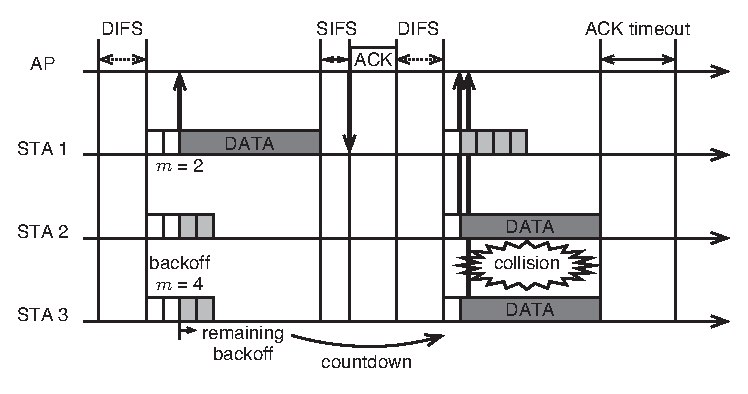
\includegraphics[width=0.8\textwidth]{fig/csmaca.eps}
					\caption{CSMA/CAの通信手順}
					\label{fig:csmaca}
				\end{center}
			\end{figure}
			\begin{figure}[t]
				\begin{center}
					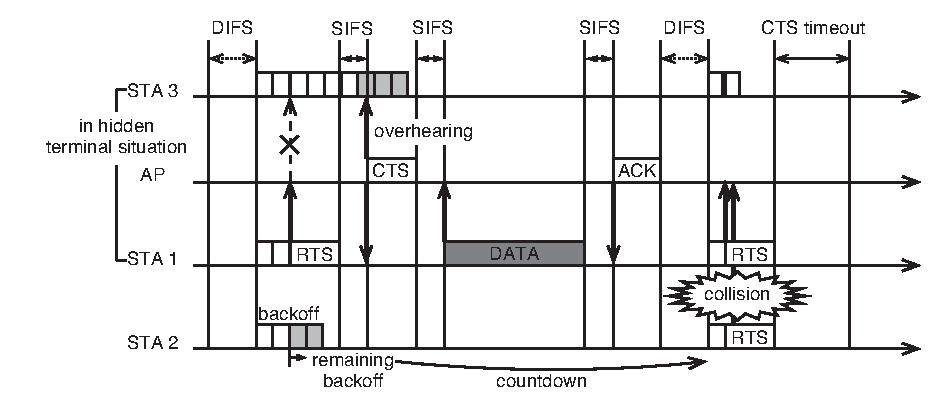
\includegraphics[width=0.8\textwidth]{fig/rtscts2.eps}
					\caption{RTS/CTSを用いたCSMA/CAでの通信手順}
					\label{fig:rtscts}
				\end{center}
			\end{figure}

		\subsubsection{フレームアグリゲーション}
			{IEEE} 802.11nで定められた無線LAN規格には,複数のデータフレームを1つにまとめて送信するアグリゲーション機能がある\cite{stdn}.
			このアグリゲーション機能について述べる前にまず,通常のデータフレームの構造を図\ref{fig:frame}\subref{fig:dataframe}に示す.
			データフレームにおいて,上位レイヤと受け渡しする部分をMSDU(MAC Service Data Unit)と呼び,
			それにMACヘッダと誤り訂正のための冗長符号であるFCS(Frame Correction Sequence)を加えた部分をMPDU(MAC Protocol Data Unit)と呼ぶ.
			アグリゲーション機能には,MSDUを連結するA-MSDU(Aggregate-MSDU)と
			MPDUを連結するA-MPDU(Aggregate-MPDU)の2種類が存在する.

			\par
			図\ref{fig:frame}\subref{fig:a-msdu}にA-MSDUのフレーム構造を,
			図\ref{fig:frame}\subref{fig:a-mpdu}にA-MPDUのフレーム構造を示す.
			ただし,アグリゲーションした際に個々のMSDU,MPDUに付加されるサブフレームヘッダは省略している.
			A-MSDUはMACヘッダやFCSを含まずにフレームを連結するのでオーバーヘッドが少なくて済むが,
			FCSが複数のMSDUに対して1つしかないため,データフレーム全体の正誤しか判定できず,
			連結したMSDUのうち1つでも受信に失敗すると連結したMSDUすべてを再送する必要がある.
			一方,A-MPDUは,1つのMSDUに対して1つのMACヘッダとFCSを持つためオーバーヘッドが大きい一方,
			MSDUごとに誤り検出が可能であるため受信に失敗したMSDUのみ再送すればよいという利点がある.
			また,A-MPDUではMSDUごとにACKが必要となるので,複数のACKをまとめたBlockACKを用いる.
			BlockACKは複数のMSDUに対して,正常に受信できたかどうかをビットマップによって示す.
			このBlockACKは通常のACKに比べてフレーム長が長い.
			IEEE802.11nではA-MSDUは連結後のMSDU部分が最大8\,kBまで,
			A-MPDUは連結後のMPDU部分が最大64\,kBまでと定められている\cite{stdn}.
			加えて,図\ref{fig:frame}\subref{fig:a-mpdu}に示すように,
			A-MPDUによってアグリゲーションされるデータフレームのMSDUは,A-MSDUによってアグリゲーションされたMSDUであってもよく,
			A-MSDUとA-MPDUによる入れ子構造が可能となっている.
			本論文では,この2つのうちA-MSDUのみを用いる.

			\begin{figure}[t]
				\begin{center}
					\subfloat[通常のデータフレームの構造]{
						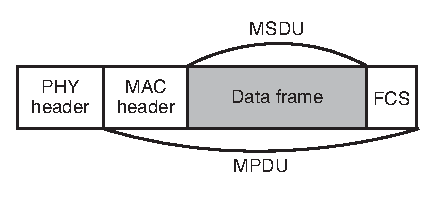
\includegraphics[width=0.3\textwidth]{fig/dataframe.eps}
						\label{fig:dataframe}}
					\\
					\subfloat[A-MSDUのフレーム構造]{
						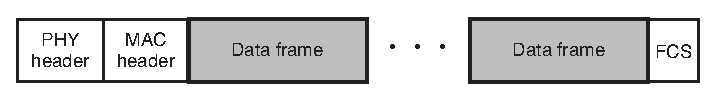
\includegraphics[width=0.569\textwidth]{fig/a-msdu.eps}
						\label{fig:a-msdu}}
					\\
					\subfloat[A-MPDUのフレーム構造]{
						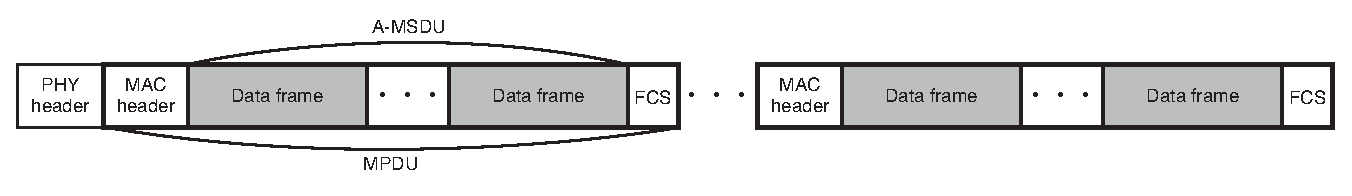
\includegraphics[width=0.871\textwidth]{fig/a-mpdu.eps}
						\label{fig:a-mpdu}}
					\caption{各データフレーム構造}
					\label{fig:frame}
				\end{center}
			\end{figure}

		\subsubsection{OFDMとOFDMA}
			IEEE 802.11無線LANでは送信信号の変調にOFDM(Orthogonal Frequency Division Multiplexing)が用いられる.
			OFDMとは,周波数利用効率を高めるため,それぞれのサブキャリアに直交性を持たせ,サブキャリア間隔を狭める方式である.
			図\ref{fig:ofdm_ofdma}\subref{fig:ofdm_ch},\subref{fig:ofdma_ch}にFDM(Frequency Division Multiplexing)と
			OFDMのサブキャリア配置の概要を示す.
			FDMでは隣接するサブキャリアが直交していないため,
			サブキャリア同士の干渉が発生しないようガードバンドと呼ばれる伝送に用いない空の帯域が必要となる.
			一方,OFDMは隣接サブキャリアが互いに直交しているため,周波数的な重なりを持っていても干渉することなく分離可能である.
			IEEE 802.11a規格では1つのチャネルに52本のサブキャリアが存在し,内4本が制御用,残り48本が伝送用として用いられる.
			\par
			OFDMAとは,複数のユーザに1つのチャネルにあるサブキャリアを割り当て並列伝送する方式である.
			OFDMではあるチャネルのすべてのサブキャリアを1つの通信に用いるのに対し,
			OFDMAではそれらのサブキャリアを複数ユーザに割り当てることで,複数ユーザとの並列伝送を実現するという違いがある.
			現在策定が進められているIEEE 802.11axにおいて,OFDMAは,短いフレームの並列伝送による周波数利用効率の向上や,
			TCP(Transmissioin Control Protocol)-ACKの遅延時間削減によるTCPスループットの向上を実現する技術として期待されている~\cite{ofdma}.

			\begin{figure}[t]
				\centering
				\subfloat[FDMのサブキャリア配置]{
					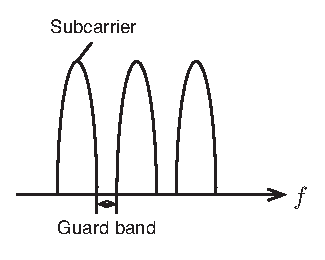
\epsfig{file=fig/ofdm_ch.eps, scale=1}
					\label{fig:ofdm_ch}
				}
				\hspace{20pt}
				\subfloat[OFDMAのサブキャリア配置]{
					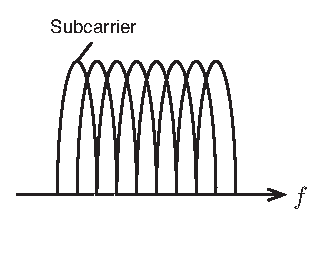
\epsfig{file=fig/ofdma_ch.eps, scale=1}
					\label{fig:ofdma_ch}
				}
				\caption{FDMとOFDMAのサブキャリアの配置}
				\label{fig:ofdm_ofdma}
			\end{figure}
	\subsection{全二重通信無線LAN}
		\subsubsection{BFD通信とUFD通信}
			本章では,全二重通信を無線LANに適用したモデルについて述べる.
			全二重通信無線LANでは,全二重通信を構成する端末の台数や位置関係によって,
			適用条件が異なるため,それらを分類しモデル化する.
			%まず,セカンダリセンダの送信先がプライマリセンダである2つの端末で構成されるモデルについて述べ,
			%次に,セカンダリセンダの送信先がプライマリセンダとは別の端末である3つの端末で構成されるモデルについて述べる.
			%さらに,後者についてキャプチャ効果を用いた適用範囲の拡大について検討した.
			\par
			図\ref{fig:model_pair}に示すように2台のAPと端末が,
			ペアとなって送受信を同じチャネルで同時に行う全二重通信をBFD(Bidirectional Full-Duplex)通信と呼ぶ.
			%MACプロトコルとしてはFD-MAC方式\cite{fdmac}を用い,
			%通信手順は図\ref{fig:fdmac_protocol}\subref{fig:pair_protocol}に示す.
			このBFD通信では,APと端末の両方が全二重通信を行っているため,
			AP,端末ともに\ref{sec:interference}節で述べる自己干渉技術が必要である.
			また,両端末の位置関係に特に制限はなく,互いに通信が可能な距離にあればよい.
			ここで,先にバックオフを終えデータフレームの送信を開始する端末をプライマリセンダ,
			それに呼応してデータフレームの送信を行う端末をセカンダリセンダと呼ぶこととする.
			よって,AP,端末ともにプライマリセンダ,セカンダリセンダの両方になりうる.

			\begin{figure}[t]
				\begin{center}
					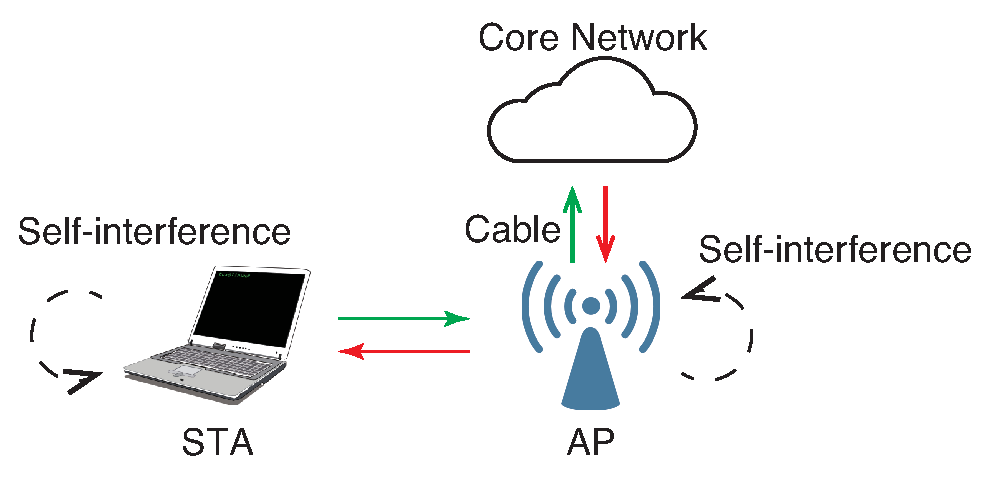
\includegraphics[width=0.5\textwidth]{fig/bfd.eps}
					\caption{BFD通信}
					\label{fig:model_pair}
				\end{center}
			\end{figure}


			\par
			図\ref{fig:model_relay}に示すようにAPの送信先端末とその端末がデータフレームを送信する端末が異なる全二重通信を
			UFD(user-multiplexing Unidirectional Full-Duplex)通信と呼ぶ.
			このUFD通信ではAPが上り通信の受信と下り通信の送信を同時に同じチャネルで行っている.
			MACプロトコルはFD-MAC方式を用い,
			通信手順は図\ref{fig:fdmac_protocol}\subref{fig:relay_protocol}に示したとおりである.
			また,自己干渉は送受信を同時に行うAPでのみ発生するため,APのみ自己干渉除去技術が利用可能であればよく,
			従来の自己干渉除去技術を持たない端末もUFD通信への参加が可能である.

			\begin{figure}[t]
				\begin{center}
					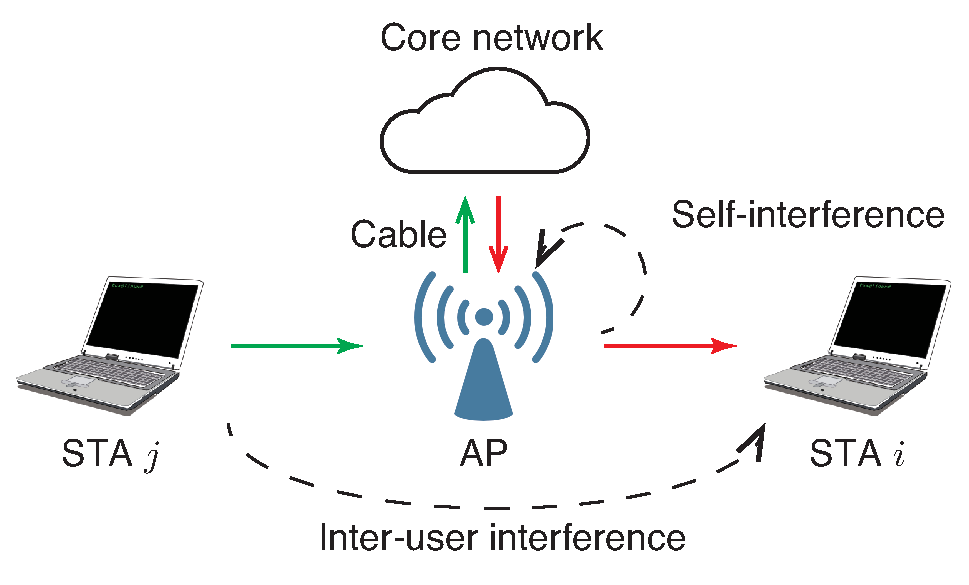
\includegraphics[width=0.5\textwidth]{fig/ufd.eps}
					\caption{UFD通信}
					\label{fig:model_relay}
				\end{center}
			\end{figure}
		\subsubsection{全二重通信無線LANにおける干渉}\label{sec:interference}
			全二重通信無線LANには従来の無線LANには存在しなかった2つの干渉が存在する.
			それは,自己干渉とユーザ間干渉である.
			\par
			自己干渉とは,ある端末が送信と受信を同じチャネルで同時に行うことによって,
			自身の送信信号が受信信号に干渉することである.
			BFD通信ではAPとSTAの両者で,UFD通信ではAPのみにおいて発生する.
			全二重通信を無線LANに適用するにあたって,この自己干渉を除去することが必要不可欠である.

			\par
			この自己干渉における干渉波にはいくつかの要素が存在する.
			遅延波のように線形性を持った要素や,回路から発生するような非線形の要素,
			さらには,増幅器や発振器から発生するランダムな要素である.
			\cite{stanford1,fdmac}では,これら複数の要素からなる自己干渉を複数の段階にわけて除去している.
			まず,1つ目は複数アンテナを用いた受動的な自己干渉除去である.
			これは,1台の端末がアンテナを複数持つ場合に,
			送受信アンテナの配置によって干渉波の伝搬損失を最大化することで
			干渉波の影響を小さくすることを目指している.
			2つ目はアナログ信号に対しての自己干渉除去である.
			自身がこれから送信するアナログ信号を遅延素子やアッテネータに通すことで,
			これから到達するであろう干渉波を生成し,それを受信信号から取り除くといったものである.
			3つ目は,前述2つの自己干渉除去を行った後,ADC(Analog Digital Convertor)を経た
			デジタル信号に対して行われる自己干渉除去である.
			ここでは,まずアナログ信号に対する干渉除去と同様に,遅延波を生成して,
			アナログ段階までで除去しきれなかった遅延波を除去する.
			さらに,テイラー展開を用いた非線形要素の一般的なモデルで非線形要素を取り除く.

			\par
			これらの方法を用いて,\cite{stanford1}では干渉波を110\,dB,\cite{fdmac}では85\,dB除去できることを示した.
			特に,110\,dBの除去が可能であるということは,例えば,送信電力が20\,dBmであった場合,
			自己干渉信号を$-$90\,dBmという端末自身が発生するノイズ・フロア程度まで落とし込むことが可能であり,
			十分実用に耐えうる値である.
			\par
			全二重通信無線LANに存在するもう1つの干渉,ユーザ間干渉とは,
			STA $j$の送信信号がもう一方のSTA $i$の受信信号に干渉を及ぼすユーザ間干渉である.
			ユーザ間干渉では,干渉を受けるSTA $i$にとって干渉波がSTA $j$の送信する未知の信号であるため,
			干渉波がある程度予測可能な自己干渉と異なり,容易に除去することができない.
			このユーザ間干渉の大きさは,干渉源端末と被干渉端末の間の距離や送信端末の送信電力に依存するため,
			ユーザ間干渉の影響を低減するために,送信を行う端末と受信を行う端末の適切な選択手法や送信電力制御手法が提案されている~\cite{fdmac3, goyal, janus, contra, promac}.
			\cite{fdmac3}ではユーザ間干渉をなくすためにSTA $i$と$j$が隠れ端末である組み合わせのみを選択し,
			\cite{goyal, janus}では事前に収集した各STAの組み合わせ毎の干渉の大きさを用いて,
			~\cite{contra}では各STAの組み合わせ毎の過去の全二重通信の成功確率を用いて組み合わせを決定する.
			また~\cite{promac}では,STAの組み合わせ毎の干渉量から上下通信の合計スループットを推定し,
			その値を最大化するSTAの組み合わせを確率的に選択する方式を提案している.
		\subsubsection{全二重通信無線LANのMACプロトコル}
			全二重通信無線LANでは複数端末が同時に送受信を行うが,
			その際,最初に送信を開始する端末をプライマリセンダ,
			プライマリセンダから受信しつつ,それに続いて同時に送信を行う端末をセカンダリセンダと呼ぶ.
			セカンダリセンダの送信先がプライマリセンダであれば,
			プライマリセンダからセカンダリセンダへの通信と,
			セカンダリセンダからプライマリセンダへの通信の全二重通信となる.
			セカンダリセンダの送信先がプライマリセンダと別の端末であれば,
			プライマリセンダからセカンダリセンダへの通信と,
			セカンダリセンダからその送信先である受信端末への通信の全二重通信となる.

			\par
			全二重通信無線LANにおけるMACプロトコルに関する既存研究として\cite{janus,contra,fdmac}があげられる.
			\cite{janus}では,Janus方式というAPによる集中制御法が提案されている.
			まず,APはProbe request packetをブロードキャストすることによって全端末に問い合わせを行う.
			これに対し各端末は,送信すべきデータフレームをがある場合にのみ
			Request flagによって送信要求を行う.
			次に,APは送信要求を行った端末に対してRequest information packetによって情報要求を行う.
			各端末は送信したいフレームの長さや互いの干渉に関する情報をAPに返送する.
			その後,それらの情報とAP自身の送信キューの情報をもとに
			各端末のデータフレーム送信タイミングや使用する伝送速度のスケジューリングを行い,
			各端末に向けてScheduling packetを送信することで,スケジュールを伝える.
			APおよび各端末は,そのスケジュールに従い順にデータフレームを送信する.
			ACKフレームの返送はすべてのデータフレームの送信が終了してから,
			再度Request acknowledgement packet によりスケジューリングを行い,
			それに従ってACK flagが返送される.
			\begin{comment}
			この一連のサイクルで使用される〜packetや〜flagは新たに定義されたフレームである.
			このプロトコルの利点は,完全なスケジューリングによって,
			制御端末であるAPに接続されている端末同士の衝突は起こらないこと,
			チャネルに空き時間が生じて半二重通信になっている時間が少ないことである.
			欠点としては,情報収集に必要なオーバヘッドが大きいことである.
			\end{comment}

			\par
			\cite{contra}では従来のCSMA/CAにビジートーン加えたContraFlow方式というMACプロトコルを用いている.
			プライマリセンダがフレームの送信を開始すると,
			それを受信し始めたセカンダリセンダは,自分が持つ過去の通信履歴に基づいて作られたリストを
			もとに送信先を決め,自分も送信を開始する.
			履歴を用いる理由は,UFD通信におけるユーザ間干渉の大きさは各端末の位置関係によって決まり,
			それによってUFD通信が可能であるかどうかが決まるためである.
			例えば,図\ref{fig:contra}のように,プライマリセンダである端末1がAPへ送信を開始した場合を考える.
			端末 1から受信を開始したAPは,自分の送信相手を端末 2,3のどちらかを選ぶことになる.
			このとき,端末 3は端末 1の信号が受信できる範囲に存在するため,
			APからの信号と衝突してしまうが,逆に,端末 2は干渉なくAPからの信号を受信できる.
			このことをAPが過去の履歴から作成したリストによって判断する.
			\begin{comment}
			このプロトコルの利点は,空き時間をビジートーンで埋めることで割り込みを防げることであり,
			欠点は,ビジートーンで空き時間は埋まっているものの,
			データフレームを送信しているわけではないので,スループットは犠牲になっている点である.
			\end{comment}

			\par
			これらJanus方式,ContraFlow方式は,従来のIEEE 802.11規格にない新たなフレームや信号,
			送信手順を用いているため,既にに広く普及している従来規格の無線LAN端末との
			後方互換性を持たず,普及には時間がかかると思われる.

			\par
			一方,\cite{fdmac}では従来のRTS/CTSを用いたFD-MAC方式によって全二重通信を実現する.
			したがって,先の2つのプロトコルとは違い,従来規格に対し後方互換性を保持しているという利点がある.
			図\ref{fig:fdmac_protocol}\subref{fig:pair_protocol}にセカンダリセンダの送信先がプライマリセンダである場合の通信手順を,
			図\ref{fig:fdmac_protocol}\subref{fig:relay_protocol}にセカンダリセンダの送信先がプライマリセンダとは別の端末である場合の通信手順を示す.
			まず,バックオフを終えた端末がプライマリセンダとなりRTSフレームを送信する.
			RTSフレームを受信したセカンダリセンダはCTSフレームを返送し,両者の同期を取る.
			その後,プライマリセンダとセカンダリセンダが同時にデータフレームを送信する.
			セカンダリセンダの送信先は,プライマリセンダかそれとは別の端末である.
			データフレームの送受信が完了した後は,同時にACKフレームを交換する.

			\par
			\cite{fdmac}では,プライマリセンダとセカンダリセンダが送信するデータフレームの時間長が
			同じであると仮定しているが,
			実際のトラヒックではデータフレームの長さは様々であり,両者のフレーム時間長は異なる.
			その結果,チャネルが空いた半二重通信の時間が発生する.
			チャネルが空くことによって生じる問題点は,以下の3つである.
			1. データフレームの送信を行わない無駄時間となりスループットが低下する.
			2. ACKがプライマリセンダが送信するデータフレームと衝突する.
			3. プライマリセンダの信号を検知できない他端末とフレームの衝突が発生する.

			\par
			例として,図\ref{fig:not_equal}に,プライマリセンダのフレーム時間長がセカンダリセンダのフレーム時間長より長い場合の通信の様子を示す.
			このような場合,セカンダリセンダは,自身のフレーム送信が終了すると,
			プライマリセンダの送信が終了するまで待機する必要があり,
			その間半二重通信となった無駄時間が生じ,スループットが低下する.
			また,受信端末が従来のHalf-duplexの端末であった場合,
			受信端末はセカンダリセンダからのデータフレームの受信を終了した後,
			SIFS時間でプライマリセンダにACKフレームを返送してしまうが,
			セカンダリセンダはプライマリセンダからのデータフレームの受信中であるので,
			セカンダリセンダにおいてプライマリセンダからのデータフレームと受信端末からのACKフレームが衝突してしまう.
			プライマリセンダが送信を終わるまで,
			受信端末がACKフレームを返送しないように改良を加えたとしても,
			プライマリセンダと受信端末が隠れ端末の関係にあると,
			受信端末はプライマリセンダの送信終了検知できず,ACKフレームの返信タイミングがわからない.
			したがって,プライマリセンダからのデータフレームと受信端末からのACKフレームが衝突してしまう.
			さらに,フレーム時間長の差とSIFSを足しあわせた時間がDIFSよりも長い場合,
			プライマリセンダの信号を受信できない端末は,
			セカンダリセンダのデータフレームの送信が終了した時点からACKフレームを送信するまでに
			チャネルがDIFSだけアイドルであったと判断し送信を開始してしまい,
			プライマリセンダのデータフレームと衝突を起こす.

			\begin{figure}[t]
				\begin{center}
					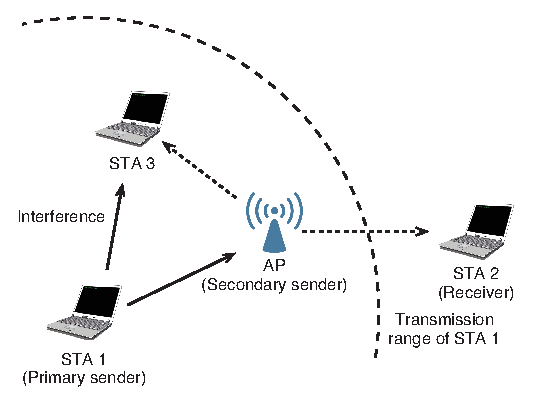
\includegraphics[width=0.7\textwidth]{fig/janus.eps}
					\caption{janusの手順}
					\label{fig:contra}
				\end{center}
			\end{figure}

			\begin{figure}[t]
				\begin{center}
					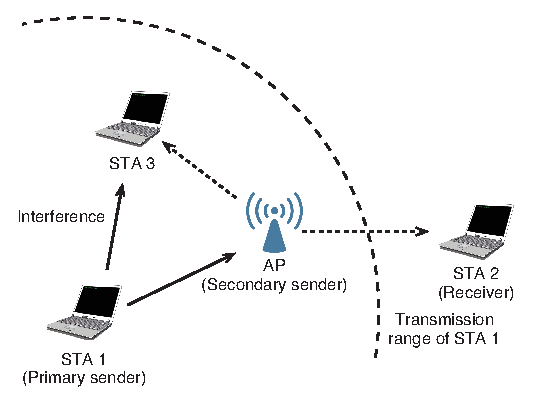
\includegraphics[width=0.5\textwidth]{fig/contra.eps}
					\caption{過去の履歴を用いた送信先の選択}
					\label{fig:contra}
				\end{center}
			\end{figure}

			\begin{figure}[t]
				\begin{center}
					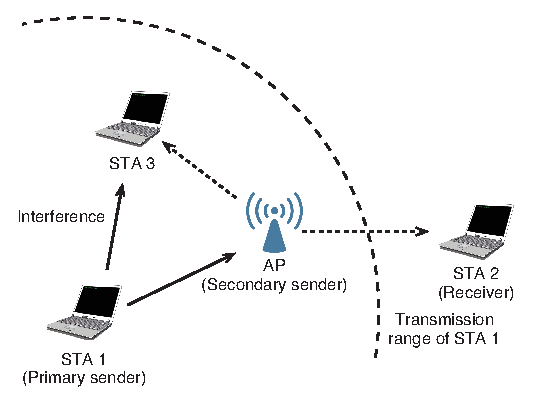
\includegraphics[width=0.7\textwidth]{fig/contra1.eps}
					\caption{ContraFlowの手順}
					\label{fig:contra}
				\end{center}
			\end{figure}

			\begin{figure}[t]
				\begin{center}
					\subfloat[セカンダリセンダがプライマリセンダに送信する場合]{
						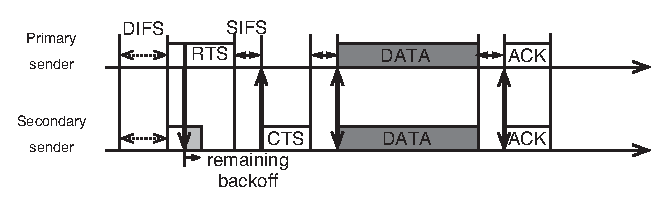
\includegraphics[width=0.8\textwidth]{fig/fdmac_protocol.eps}
						\label{fig:pair_protocol}}
					\\
					\subfloat[セカンダリセンダが別の端末に送信する場合]{
						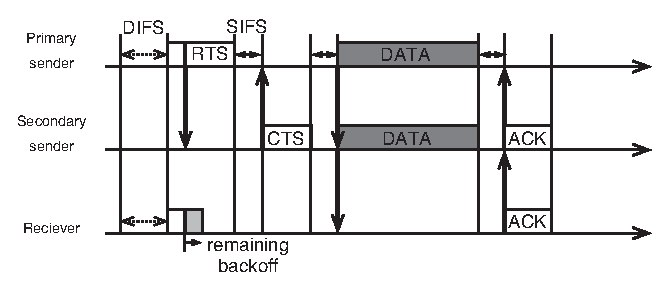
\includegraphics[width=0.8\textwidth]{fig/relay_protocol.eps}
						\label{fig:relay_protocol}}
					\caption{既存研究\cite{fdmac}による全二重通信無線LANのMACプロトコル}
					\label{fig:fdmac_protocol}
				\end{center}
			\end{figure}

			\begin{figure}[t]
				\begin{center}
					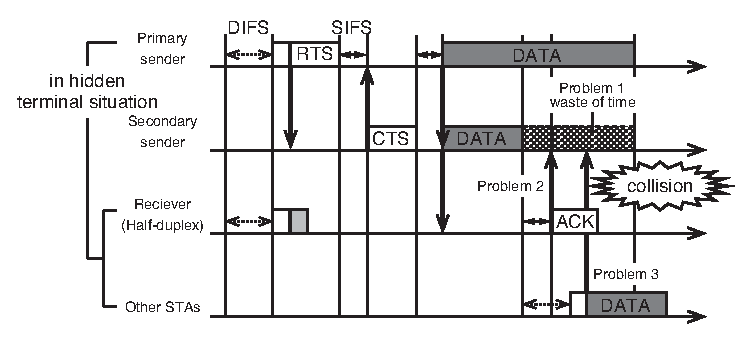
\includegraphics[width=0.8\textwidth]{fig/relay_not_equal2.eps}
					\caption{フレーム時間長が揃っていない場合の問題点}
					\label{fig:not_equal}
				\end{center}
			\end{figure}

		\subsubsection{UFD通信通信におけるSTA選択}
			\label{sec:interference}項で述べた通り,UFD通信における\cite{promac}ユーザ間干渉は自己干渉のように除去できないため,
			適切なSTAの組み合わせを選択する必要がある.
			本章では,ユーザ間干渉の低減に向けた既存研究~\cite{promac}について述べる.
			\par
			\cite{promac}はシステムスループットの期待値を目的関数とし,
			各STAの組み合わせの選択確率を変数とした最適化問題を解くことで各STAの選択確率を決定し,確率的なSTA選択を行う.
			\par
			まず,UFD通信を行うSTAの組み合わせの集合${\mathcal C}_{\rm full}$を式\eqref{eq:cfull}に示す.
			\begin{equation}
				{\mathcal C}_{\rm full} \coloneqq \{\sij : i,j\in{\mathcal N},\ i\neq j,\ r^{\sij}_{\rm d},\ r^{\sij}_{\rm u}>\epsilon\} \label{eq:cfull}
			\end{equation}
			ただし,$r_{\rm d}^{\sij}$,$r_{\rm u}^{\sij}$はそれぞれAPからSTA $i$への下りの実効スループット,
			STA $j$からAPへの上りの実効スループットであり,$\epsilon$はスループットが0に近くなるようなSTAの組み合わせを除くためのしきい値である.
			${\mathcal C}_{\rm full}$の全組み合わせに対して,上り下り通信それぞれの実効スループット$\rd$,$\ru$を推定し,$\rij=\rd + \ru$とする.
			実効スループットの推定には,
			上り下り通信のそれぞれのSINR(Signal-to-Interference plus Noise power Ratio)から求めた以下のシャノン容量を用いる.
			\begin{equation}
				{\rm Shannon\ capacity}=B\log_2(1+{\rm SINR}) \label{eq:capacity}
			\end{equation}
			ただし,$B$は通信に用いる帯域幅である.
			実行スループットの推定には干渉の影響が含まれ,干渉が小さいほど$\rij$は大きくなる.
			更に,半二重通信の組み合わせ
			\begin{equation}
				{\mathcal C}_{\rm half} \coloneqq \{\sij : ij=0,\ \rij >\epsilon\}
			\end{equation}
			に対しても実効スループット$\rij$を推定する.
			ここで,${\mathcal C} = {\mathcal C}_{\rm full} \cup {\mathcal C}_{\rm half}$とし,
			\begin{align}
				{\mathcal N}_i &= \{i|(i,\ j)\in{\mathcal C}\}\\
				{\mathcal N}_j &= \{j|(i,\ j)\in{\mathcal C}\}
			\end{align}
			得られた$\rij$に基づいて以下の最適化問題を解き,確率$\pij$を得る.
			\begin{align}
				&{\mathcal P}_1: && {\rm max} \sum_{(i,\ j)\in{\mathcal C}} p^{(i,\ j)}r^{(i,\ j)} &&&&&& \label{eq:p1}\\
				&{\rm subject\ to} && \sum_{j\in\{j:(i,\ j)\in{\mathcal C}\}} p^{(i,\ j)} \geq \eta_{\rm d}^{(i)},\ \forall i\in {\mathcal N} \label{eq:pd} \\
				&&& \sum_{i\in\{i:(i,\ j)\in{\mathcal C}\}} p^{(i,\ j)} \geq \eta_{\rm u}^{(j)},\ \forall j\in {\mathcal N} \label{eq:pu}\\
				&&& \sum_{j\in\{j:(i,\ j)\in{\mathcal C}\}} p^{(i,\ j)}=1 \\
				&{\rm variables:} &&p^{(i,\ j)} \in {\mathbb R}_{\geq 0},\ \forall(i,\ j)\in {\mathcal C} \nonumber
			\end{align}
			実行スループット$\rij$は干渉が小さいほど大きくなり,大きい$\rij$を持つSTAの組み合わせほど$p^{\sij}$が大きくなる.
			制約条件の式\eqref{eq:pd},\eqref{eq:pu}は各STAが下り通信の送信先,あるいは,上り通信の送信元となる確率が0とならないように下限を定めるためのものである.
			$\eta_{\rm d}^{(i)}$はSTA $i$が下り通信の送信先となる確率$p_{\rm d}^{(i)}=\sum_{j\in\{j:(i,\ j)\in{\mathcal C}\}} p^{(i,\ j)}$
			の最低値であり,STA $i$への下り通信のトラヒックに比例した値が設定される.
			同様に,$\eta_{\rm u}^{(j)}$は$p_{\rm u}^{(j)}=\sum_{i\in\{i:(i,\ j)\in{\mathcal C}\}} p^{(i,\ j)}$
			の最低値であり,STA $j$の上り通信のトラヒックに比例した値が設定される.
			\par
			また,以下の条件が満たされるとき必ず解が得られることが示されている.
			\begin{align}
				r_{\rm d}^{(i,\ 0)} >\epsilon,\ \forall i\in\mN \\
				r_{\rm u}^{(0,\ j)} >\epsilon,\ \forall j\in\mN \\
				\sum_{i\in\mN}\eta_{\rm d}^{(i)} + \sum_{j\in\mN}\eta_{\rm u}^{(j)} =1 \label{eq:feasible}
			\end{align}
			なお,この最適化問題は毎回あるいは複数のビーコン信号周期毎に解かれ,更新された確率$\pij$はビーコンフレームによってSTAに通知される.
			\par
			次に,得られた$\pij$を用いてSTA $i$,$j$を決定する方法を述べる.
			APは
			\begin{equation}
				p_{\rm d}^{(i)}= \sum_{j\in\{j:(i,\ j)\in{\mathcal C}\}}p^{(i,\ j)},\ \forall i \in \{0\}\cup{\mathcal N}
			\end{equation}
			によって各STAが下り通信の送信先となる確率$p_{\rm d}^{(i)}$を求め,$p_{\rm d}^{(i)}$に従って確率的に送信先STA $i$を選択する.
			続いてSTA $j$の上り通信の送信権について述べる.
			APからの下り通信を受信するSTA $i$の決定後,APはSTA $i$へ送信するフレームのヘッダ部分のみを送信し,
			全STAに下り通信の送信先がSTA $i$であることを通知する.
			STA $i$以外のすべてのSTAは以下の条件付き確率
			\begin{equation}
				p_{\rm u}^{\sij} = P(j\ {\rm wins\ uplink}\mid{\rm AP\ sends\ to}\ i)=\pij / p_{\rm d}^{(i)} \label{eq:win}
			\end{equation}
			を計算する.
			これはAPがSTA $i$へ下り通信を行うことが決まった上で自身がAPへの上り通信の送信権を獲得する確率を意味する.
			この条件付き確率をもとに,コンテンションウィンドウサイズ${\rm CW}^{\sij}_{\rm u}$を
			\begin{equation}
				{\rm CW}^{\sij}_{\rm u} = \lceil 1/p_{\rm u}^{\sij} \rceil
			\end{equation}
			と設定する.
			ただし,$\lceil x \rceil$は$x$を超えない最大の整数である.
			各STAは$[0,\ {\rm CW}^{\sij}_{\rm u}]$の一様分布から生成されるバックオフカウンタ$w_{\rm u}^{\sij}$を設定し,
			CSMA/CAのバックオフアルゴリズムを用いてバックオフカウンタを1ずつ減らす.
			その結果,最初にカウンタが0となったSTAが上り通信を行う.
			この方法により,$p_{\rm u}^{(j)}$が大きいSTA,つまり式\eqref{eq:p1},\eqref{eq:win}より$r^{\sij}$が大きいSTAほど${\rm CW}^{\sij}_{\rm u}$が小さくなり,
			送信権を得やすくなる.

			\par
			式\eqref{eq:p1}からわかるように~\cite{promac}によるSTA決定手法では,
			STA $i$,$j$間のユーザ間干渉が小さくスループット$\rij$が大きい組み合わせほど選ばれる確率が高くなるため,
			一部の組み合わせに確率が集中し,特にSTAの上り通信において不公平性を生じる.
			図\ref{fig:numtx}にSTA台数を$N=50$としたシステムで
			従来方式による各STAの上り通信送信回数のシミュレーション結果を示す.
			この結果から一部のSTAが上り通信を行うSTAになる確率が高く,送信回数が突出して多くなり,
			送信機会に関する不公平性が生じていることがわかる.
			加えて,STA間の遅延要求の違いについては議論されておらず,低遅延を要求するSTAが混在し
			そのSTAの実効スループットが低い場合,
			そのSTAが送信機会を得るまでに大きな遅延が生じる可能性がある.
			本稿では,この2つの問題点に関して解決を図り,QoSの向上を目指す.
			\par
			また,UFD通信は半二重通信に比べてSTAの遅延時間を増大させるという問題がある.
			これは,図\ref{fig:problem}に示すように,UFD通信ではユーザ間干渉により伝送速度が低下するため一回の送信時間が増加し,
			かつ,下り通信の送信頻度が増加するため,半二重通信と比較してSTAの送信頻度が低下するためである.
			上り通信の遅延時間の増大は,TCP下り通信におけるTCP-ACKパケットの遅延を増加させ,
			結果的にTCPスループットの低下が生じる~\cite{rtt}.

			\begin{figure}[t]
				\centering
				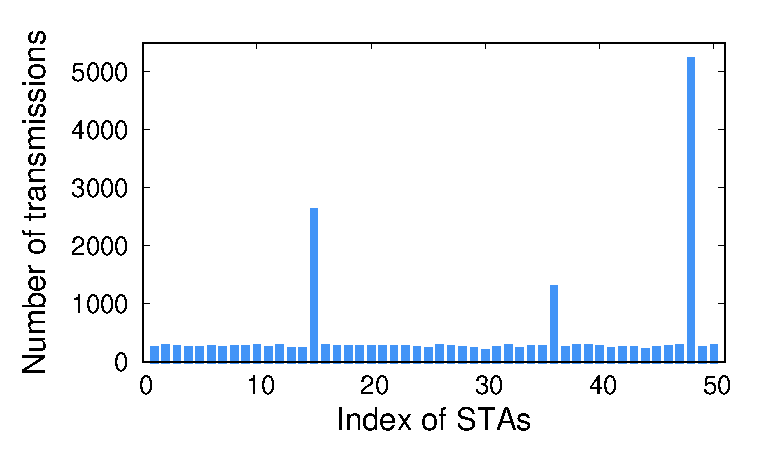
\epsfig{file=graph/numtx.eps, scale=0.8}
				\caption{従来方式~\cite{promac}によるSTAの送信回数の分布}
				\label{fig:numtx}
			\end{figure}

			\begin{figure}[t]
				\centering
				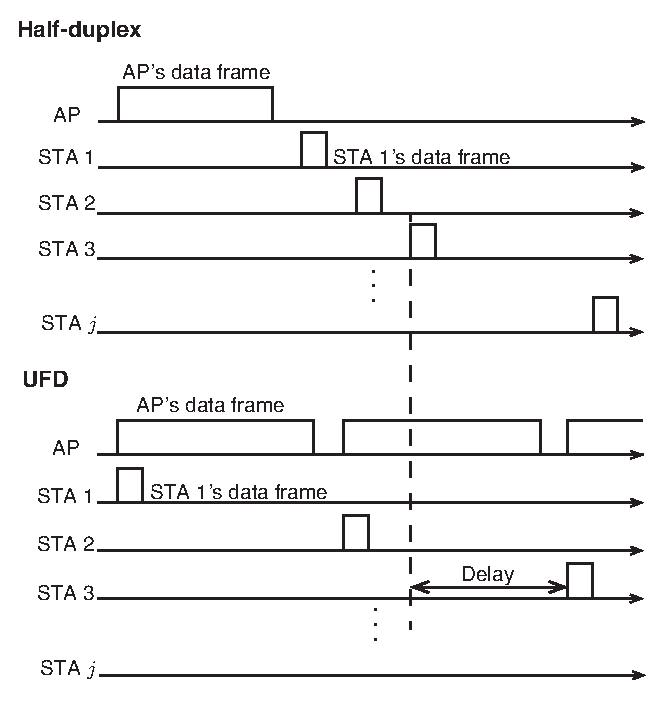
\epsfig{file=fig/problem.eps, scale=0.8}
				\caption{半二重通信とUFD通信におけるSTAの送信機会}
				\label{fig:problem}
			\end{figure}


\section{提案方式}
	\subsection{フレーム時間長最適化}
		本節では無駄時間削減のためにフレーム時間長最適化を提案する.
		提案方式ではFD-MAC\cite{fdmac}を用いて最適化を行う.
		最適化はセカンダリセンダが送信するデータフレームの時間長を,プライマリセンダが送信予定のデータフレームの時間長に揃えることによって行う.
		そのためにはセカンダリセンダがプライマリセンダが送信するデータフレームの時間長を知る必要がある.
		以下,セカンダリセンダがプライマリセンダのデータフレームの時間長を知る手法,さらに,得られた時間長に対して自身のデータフレームの時間長を最適化する手法について述べる.
		\par
		FD-MACでは送信権を獲得した端末がプライマリセンダとしてRTSフレームを送信する.
		セカンダリセンダはこのRTSフレームに含まれる情報からプライマリセンダが送信予定のデータフレームの時間長を知ることができる.
		RTSフレームにはデュレーションフィールドと呼ばれる部分があり,そこには以下の値が格納されている.
		\begin{equation}
			{\rm duration\ value} = {\rm SIFS} \times 3 + T_{{\rm CTS}} + T_{{\rm data}} + T_{{\rm ACK}}
		\end{equation}
		ただし,$T_{\rm CTS}$ はCTSフレームを,$T_{\rm data}$ はデータフレームを,$T_{\rm ACK}$はACKフレームを送信するのにかかる時間である.
		この値はRTSフレームの送信終了からACKフレームの送信終了までの時間を示す.
		また,CTSフレームとACKフレームのフレーム長はIEEE 802.11規格によって定められている.
		このことと上式を合わせると,セカンダリセンダはデュレーションフィールドの値から固定長である$T_{\rm CTS}$,$T_{\rm data}$ ,$T_{\rm ACK}$を減算することでプライマリセンダが送信するデータフレームの時間長を知ることができる.
		\par
		次に,セカンダリセンダは以下の二つの段階によって自身が送信するデータフレームの時間長をプライマリセンダが送信するデータフレームの時間長に揃える.
		前述の通り,セカンダリセンダはプライマリセンダが送信するRTSフレームによって最適化の目標値となるプライマリセンダのフレーム時間長を知る.
		そのため,最適化に用いることができる時間は,最大でもRTSフレームを受信し終わってからデータフレームの送信を開始するまでである.
		この限られた時間内に最適化を終えるためには計算時間をできるだけ短くすることが必要である,
		提案手法ではセカンダリセンダのバッファにあるデータフレームを複数個アグリゲーションすることで,
		プライマリセンダが送信するデータフレームとの時間長の差を最小化するが,
		アグリゲーションするデータフレームの組み合わせの数はバッファに存在するデータフレームの数と最適化の目標値に依存する.
		最適化の目標値,つまり,プライマリセンダのデータフレーム時間長が大きい場合は,
		用いることができるデータフレームが多くなり,その組み合わせの数は膨大になる.
		一方,最適化の目標値が小さい場合は,目標値よりも長いデータフレームは用いることができないため,組み合わせの数は少なくなる.
		そこで,提案手法では最適化を粗い調整と細かい調整の2つの段階に分ける.
		第一段階の粗い調整によって大まかにフレーム時間長を調整した後,細かな調整によって残ったフレーム時間長の差を最小化する.
		\par
		第一段階の粗い調整ではセカンダリセンダはバッファの先頭から順に$m$個のデータフレームをアグリゲーションする.
		$m$は以下の式によって決定される.
		\begin{align}
			&\argmax_m L^{\rm f} = \sum_{i = 1}^{m} L_i \\
			&{\rm subject \ to} \qquad  L^{\rm p} \geq \sum_{i = 1}^{m} L_i
		\end{align}
		$L^{\rm f}$は一段階目でアグリゲーションされたデータフレームの長さであり,$L_i$はバッファの$i$番目のデータフレームの長さ,
		そして,$L^{\rm p}$はプライマリセンダが送信するデータフレームの長さである.
		これは,バッファの先頭から順にプライマリセンダのデータフレーム時間長を超えないところまでアグリゲーションしていくことを示す.
		この第一段階によって,セカンダリセンダのフレーム時間長は大まかにプライマリセンダのフレーム時間長に揃えられる.
		\par
		第二段階では,第一段階終了後に残っているフレーム時間長の差を最小化する.
		前述したとおり,プライマリセンダのデータフレーム時間長全てではなく,
		残った差を最適化の目標値とすることで計算時間の削減を達成している.
		加えて,この第二段階で用いることができるデータフレーム数の上限を$n$とすることで組み合わせの総数を減少させ,さらなる計算時間の削減目指す.
		セカンダリセンダは以下の最適化問題を解くことによって,アグリゲーションに用いるフレームの集合${\mathcal F}^{\rm s}$を決定する.
		\begin{align}
			&{\mathcal F}^{\rm s} = \argmin_{{\mathcal X} \subseteq {\mathcal F}} L^{\rm p} - L^{\rm f} - \sum_{i \in {\mathcal X}}L_{i} \\
			&{\rm subject \ to} \qquad |{\mathcal X}| \leq n \\
			&\;\;\qquad\qquad\qquad L^{\rm p} - L^{\rm f} - \sum_{i \in {\mathcal X}} L_{i} \geq 0
		\end{align}
		ただし${\mathcal F}$はセカンダリセンダのバッファに残っているデータフレームの集合である.
		第二段階で用いることができるデータフレーム数の上限$n$を小さくするほど計算時間が短くなる一方,最適化の度合いは減少する.
		\par
		図\ref{fig:opti}にセカンダリセンダによるフレーム時間長最適化の一例を示す.
		第一段階では,バッファの先頭から$m+1$番目までのデータフレームをアグリゲーションするとプライマリセンダが送信するデータフレームの時間長を超えてしまことから,第一段階ではバッファの先頭から$m$番目までのデータフレームを用いることが決まる.
		第二段階では,残ったプライマリセンダのフレーム時間長との差を$n$個以下のフレームで埋める.
		このとき,バッファの$m+2$番目から最後までのデータフレームが用いられる.
		これら二つの段階で決定したデータフレームをアグリゲーションしたものがセカンダリセンダが送信するデータフレームとなる.
		\par

		\begin{figure}[t]
			\begin{center}
				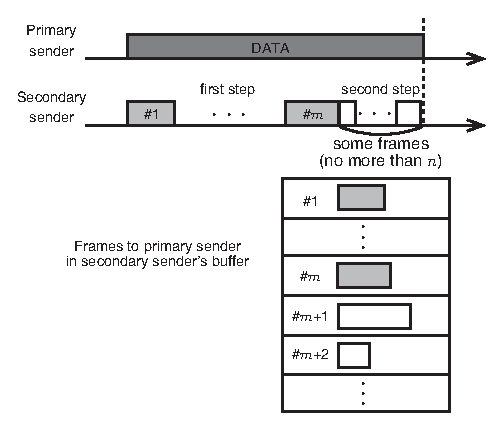
\includegraphics[width=0.39\textwidth]{fig/opti.eps}
				\caption{How to optimize frame length on secondary sender.}
				\label{fig:opti}
			\end{center}
		\end{figure}

	\subsection{UFD通信におけるSTA選択}
		\subsubsection{公平性の改善}\label{sec:fair}
			前章に述べたように従来方式のMACプロトコルでは干渉が小さい組み合わせが選ばれやすく,
			特定のSTAに送信機会が偏るという課題がある.
			この問題を解決をするため以下の目的関数を提案する.
			\begin{equation}
				{\mathcal P}_2: {\rm max} \sum_{(i,\ j)\in{\mathcal C}} p^{(i,\ j)}r^{(i,\ j)}(d^{(j)})^{\alpha} 	\label{eq:p2}
			\end{equation}
			$d^{(j)}$は待機時間であり,STA $j$のバッファの先頭にフレームが到着してから現在時刻までの時間とする.
			この待機時間の項を追加することで,待機時間が長いSTA,つまり,送信機会を得られていないSTAを含んだ組み合わせが選ばれる確率が高くなり,
			送信機会の均等化を図ることができる.
			また,待機時間は飽和トラヒックである限りは前回の送信時刻からの経過時間と同じであるため,
			新たに各STAの待機時間情報を収集する必要はなく,APが各STA毎に最新の送信時刻を記憶することで,
			現在時刻との差として得られる.
			追加する項として各STAの平均送信間隔や送信回数そのものを選択しない理由は,
			両者はいずれも積算値であるため,新たにSTAがAPに接続された場合平均送信間隔は定義できず,
			送信回数は0であるため選択される確率が極端に高くなり短期的な不公平性が生じる可能性があるためである.
			\par
			公平性の改善を行うと,公平性の改善を行わない場合に比べて比較的干渉の多いSTAの組み合わせが選ばれることが多くなり,
			システムスループットの低下が考えられる.
			そのため,公平性の改善とシステムスループットの低下のトレードオフを調整可能とするための重み係数$\alpha\geq 0$を導入する.
			$\alpha$が小さい場合は待機時間$d^{(j)}$の影響が小さくなるため,システムスループットが高くなり公平性は低くなる.
			逆に$\alpha$が大きい場合は待機時間$d^{(j)}$の影響が大きくなり,システムスループットが大きく低下するかわりに公平性が高くなる.
		\subsubsection{低遅延を要求するSTAのQoSの向上}
			本節では,システム全体の公平性を改善した上で,更に低遅延を要求するSTAのQoS改善を行う提案方式について述べる.
			低遅延を要求するSTAのQoSを向上させるためには,
			上り通信を行う確率$p_{\rm u}^{(j)}$を大きくし,送信機会を増加させればよい.
			これを実現するために,式\eqref{eq:pu}において$p_{\rm u}^{(j)}$の最低値を決定している$\etau$の設定法を検討する.
			従来方式では,STA $j$の上り通信のトラヒックに比例した値が$\etau$には設定されていが,
			提案方式では以下のように新たな${\hat \eta}_{\rm u}^{(j)}$を設定する.
			\begin{align}
				&{\hat \eta}_{\rm u}^{(j)} = \etau -x_j,\ \forall j \in {\overline {\mathcal D}} \label{eq:etadbar}\\
				&{\hat \eta}_{\rm u}^{(j)} = \etau + x_j',\ \forall j \in {\mathcal D} \label{eq:etad}\\
				%&x_j >0,\ \forall j\in{\overline {\mathcal D}} \\
				%&\etau > x_j,\ \forall j\in{\overline {\mathcal D}} \\
				%&x_j'>0,\ \forall j\in{\mathcal D} \\
				&\sum_{j\in{\overline {\mathcal D}}} x_j = \sum_{j\in{\mathcal D}} x_j' \label{eq:sub}
				\end{align}
			低遅延を要求していないSTAの$\etau$を$x_j$だけ小さくし,
			低遅延を要求するSTAの$\etau$を$x_j'$だけ大きくする.
			ただし,$0<x_j<\etau,\ \forall j\in{{\overline {\mathcal D}}}$であり,$0<x_j',\ \forall j\in{\mathcal D}$とする.
			また,式\eqref{eq:sub}は式\eqref{eq:feasible}を満たし可解性を失わないための条件である.
			提案方式では以上のように新たに設定された${\hat \eta}_{\rm u}^{(j)}$を最適化問題の制約条件である式\eqref{eq:pu}に用いる.
			これによって,低遅延を要求するSTAの送信機会が増加し送信間隔が短くなることで遅延時間が短縮されQoSが改善される.
		\subsection{上りOFDMAによるUFD通信通信の遅延時間削減}
			本節では,遅延時間削減に向け,UFD通信の上り通信へOFDMAを適用した無線LANと本無線LANにおける送受信STA選択手法を提案する.
			図\ref{fig:ofdma}にシステムモデルを示す.
			提案方式では,OFDMA導入により,送受信STAの選択において複数の上り通信STAを選択可能とし,
			STAの送信機会を向上することで遅延を削減する.
			本論文では,~\cite{promac_fair}で提案する送受信STA選択最適化問題を拡張し,上りOFDMAに対応したSTA選択を可能とする.
			提案手法では,半二重通信,UFD通信,上りOFMDA,UFD通信と上りOFDMAの組み合わせの4つの通信方式を適応的に切り替え,STA選択を行う.
			送受信STA組を適応的に選択することで,干渉が大きくUFD通信を行えないような位置にあるSTAは半二重通信を行い,
			干渉が小さく,大きなスループットを期待できるSTAにはUFD通信を用い,
			多くのSTAへ送信機会を与えたい場合はOFDMAを用いるといったような状況に応じた制御が可能となる.
			\begin{figure}[t]
				\centering
				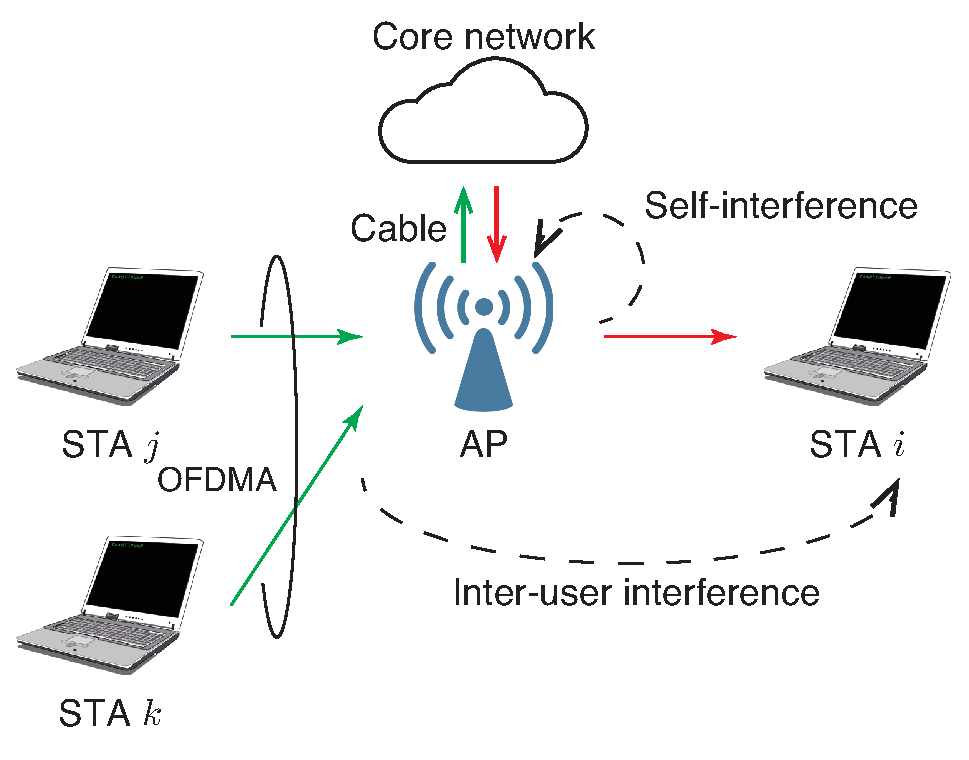
\epsfig{file=fig/ofdma.eps, scale=0.35}
				\caption{UFD通信とOFDMAの組み合わせ}
				\label{fig:ofdma}
			\end{figure}
			\subsubsection{STA選択手法の拡張}
				本節では,遅延時間の増大を防ぐため,上り通信をOFDMAを用いて多重化することを提案する.
				OFDMAを用いてSTAの送信機会を増加させることで遅延時間を削減する.
				STA決定手法は従来方式~\cite{promac_fair}における手法をOFDMAを適用できるように拡張する.
				また,本章で述べる部分以外のMAC(Media Access Control)プロトコルは~\cite{promac}に従う.
				\par
				ただし,OFDMAによる多重化は簡単のため二多重までとし,半二重通信,UFD通信で用いるチャネルを2台のSTAが二等分して用いる.
				この$N$台のSTAの中から,図\ref{fig:ofdma}のようにAPからの下り通信を受信するSTA $i$と,
				APへの上り通信を行うSTA $j$,$k$を選び出す.
				このとき,STAの組み合わせを$\sijk$と表現し,$i,\ j,\ k \in \{0\}\cup \mN$とする.
				STAは自己干渉除去技術を持たずBFD通信はできないとし,$i\neq0$のときには$i\neq j$かつ$i\neq k$とする.
				また,$i$,$j$,$k$の全てが0になることはないものとする.
				$i$,$j$,$k$のそれぞれが取る値によって以下の通信方式を定義し,切り替え可能であるものとする.
				\begin{itemize}%\setlength{\leftskip}{10pt}
					\item ($i=0\land jk=0\land j+k\neq0)\lor (i=0\land j=k\neq0)$\par
					\hspace*{15pt}上りの半二重通信
					\item $i\neq0\land j=k=0$\par
					\hspace*{15pt}下りの半二重通信
					\item $(i\neq0\land jk=0 \land j+k\neq0)\lor(i\neq0\land j=k\neq0)$\par
					\hspace*{15pt}UFD通信
					\item $i=0\land jk\neq0 \land j\neq k$\par
					\hspace*{15pt}上りOFDMA
					\item $i\neq0 \land jk\neq0 \land j\neq k$\par
					\hspace*{15pt}OFDMAとUFD通信の組み合わせ
				\end{itemize}
				\par

				%\subsection{送受信STA組決定手法の概要}\label{sec:opt}
				\begin{figure}[t]
					\centering
					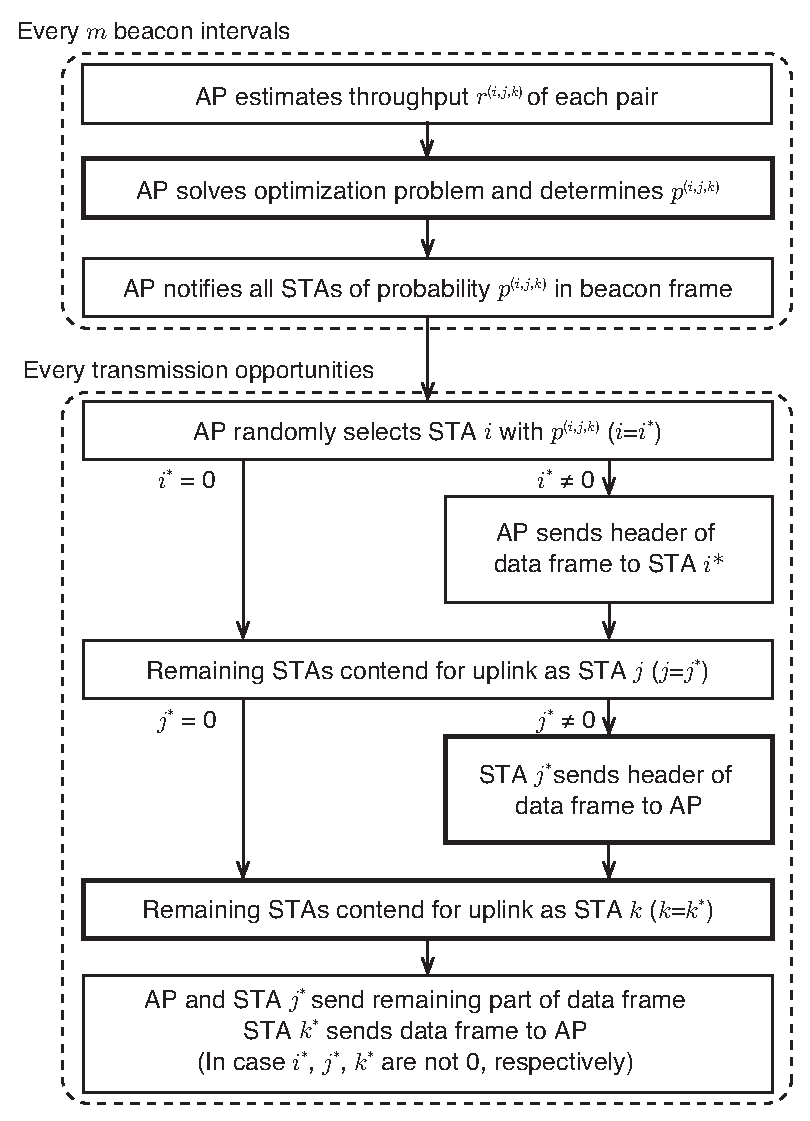
\epsfig{file=fig/proccess.eps, scale=0.7}
					\caption{送受信STA選択手法の手順}
					\label{fig:process}
				\end{figure}
				%まず,STAの組み合わせの集合${\mathcal C}_{\rm half}$,${\mathcal C}_{\rm UFD}$,${\mathcal C}_{\rm OFDMA}$,${\mathcal C}_{\rm OFDMA-UFD}$,${\mathcal C}$を以下のように定義する.
				%\begin{align}
				%	&{\mathcal C}_{\rm half} \coloneqq \{\sijk : i=0\cap ((jk=0 \cap j+k\neq0) \cup(j=k\neq0)),\ \rijk >\epsilon\} \\
				%	&{\mathcal C}_{\rm UFD} \coloneqq \{\sijk : i,j\in{\mathcal N},\ i\neq j,\ r^{\sij}_{\rm d},\ r^{\sij}_{\rm u}>\epsilon\} \\
				%	&{\mathcal C}_{\rm OFDMA} \coloneqq \{\sijk : i=0,\ jk\neq0\in{\mathcal N},\ r^{\sij}_{\rm d},\ r^{\sij}_{\rm u}>\epsilon\}
				%\end{align}
				本手法の手順は図\ref{fig:process}の通りである.
				太枠で示した部分が,OFDMAの適用にあたって拡張を行った部分である.
				本手法は各STA組毎の干渉の大きさや各STAの遅延時間をもとに,通信方式の選択と送受信を行うSTA組を適応的に決定することが目的である.
				そのため,まずAPは全STA組に対してその組み合わせで通信が行われた場合のスループットを推定する.
				また,各STAの送信待機時間を事前に収集しておく.
				ただし,送信待機時間とは各STAにおいてあるデータフレームがバッファの先頭に到着してから現在時刻までの経過時間である.
				APは推定されたスループットと各STAの送信待機時間を用いて最適化問題を解き,各STA組で通信が行われる確率を求める.
				最適化問題の目的関数は,システムスループットを大きくし,かつ,STAの遅延時間を削減するため,
				前述の推定スループットが大きいSTA組や送信待機時間が長いSTAを含むSTA組が選ばれやすくなるよう設計する.
				推定スループットは干渉の大きさや用いる伝送速度によって変化し,送信待機時間はSTAが送信を行う度に変化する上,
				STAの増減も起こる.
				そういった状況の変化に対応するために,APは定期的にスループットの再推定と送信待機時間の再収集を行い,
				最適化問題を解き直すことで確率を更新する.
				得られた確率はビーコンフレームによって全てのSTAへ通知される.
				\par
				次に,得られた確率を用いてSTA組を決定する.
				APは下り通信の送信先となるSTA $i$を確率的に決定する.
				選ばれたSTAをSTA $i^*$とし,APは送信先がSTA $i^*$であることを通知するため,データフレームのヘッダ部分を送信する.
				続いて,全てのSTAはAPから通知された確率をもとにコンテンションウィンドウを設定し,
				CSMA/CA (Carrier Sence Multiple Access with Collision Avoidance)のバックオフアルゴリズムを用いた競合を行い,
				STA $j$,$k$が順に決定される.
				決定したSTAをそれぞれSTA $j^*$,$k^*$とし,
				STA $j^*$は自身が送信権を獲得したことを通知するため,データフレームのヘッダ部分を送信する.
				最後に,APとSTA $j^*$はデータフレームの残りの部分を,STA $k^*$はデータフレームを送信する.

		\subsubsection{送受信STA組決定手法の詳細}
			本節では前節で述べた各手順について詳細を述べる.
			従来方式~\cite{promac_fair}に対しては,OFDMAを適用しSTA $k$を追加するために,最適化問題の拡張とSTA $k$の決定手順追加がなされている.
			\par
			まず,UFD通信の場合,半二重通信の場合の組み合わせ集合を前節と同様に
			\begin{align}
				{\mathcal C}_{\rm full} \coloneqq \{\sij : i,j\in{\mathcal N},\ i\neq j,\ r^{\sij}_{\rm d},\ r^{\sij}_{\rm u}>\epsilon\} \label{eq:cfull}\\
				{\mathcal C}_{\rm half} \coloneqq \{\sij : i,j\in{\mathcal N},\ i\neq j,\ r^{\sij}_{\rm d},\ r^{\sij}_{\rm u}>\epsilon\} \label{eq:cfull}
			\end{align}
			とする.さらに,OFDMAの組み合わせ,UFD+OFDMAの組み合わせを新たに,
			\begin{align}
				{\mathcal C}_{\rm ofdma} \coloneqq \{\sij : i,j\in{\mathcal N},\ i\neq j,\ r^{\sij}_{\rm d},\ r^{\sij}_{\rm u}>\epsilon\} \label{eq:cfull}\\
				{\mathcal C}_{\rm ufd+ofdma} \coloneqq \{\sij : i,j\in{\mathcal N},\ i\neq j,\ r^{\sij}_{\rm d},\ r^{\sij}_{\rm u}>\epsilon\} \label{eq:cfull}
			\end{align}
			とする.さらにこれらの和集合を${\mathcal C} = {\mathcal C}_{\rm full} \cup {\mathcal C}_{\rm half}\cup {\mathcal C}_{\rm ofdma}\cup {\mathcal C}_{\rm ufd+ofdma}$
			とする.
			\begin{equation}
				{\mathcal C}_{\rm full} \coloneqq \{\sij : i,j\in{\mathcal N},\ i\neq j,\ r^{\sij}_{\rm d},\ r^{\sij}_{\rm u}>\epsilon\} \label{eq:cfull}
			\end{equation}
			まず,APは全ての組み合わせ$(i,j,k)$に対してスループット$r^{(i,j,k)}_{\rm d}$,$r^{(i,j,k)}_{\rm u1}$,$r^{(i,j,k)}_{\rm u2}$を推定する.
			ただし,$r^{(i,j,k)}_{\rm d}$はAPからSTA $i$への下り通信の推定スループット,$r^{(i,j,k)}_{\rm u1}$,$r^{(i,j,k)}_{\rm u2}$はSTA $j$,$k$による上り通信の推定スループットである.
			ここで,全組み合わせの集合から最低伝送速度の所要SINRを満たさない通信が含まれている組み合わせを除外した集合を$\mthc$とし,
			$\mthc$の要素$\sijk$に含まれる$i$,$j$,$k$の集合をそれぞれ$\mthni$,$\mthnj$,$\mthnk\subseteq \{0\}\cup{\mathcal N}$とする.
			APは$\rijk=r^{(i,j,k)}_{\rm d}+r^{(i,j,k)}_{\rm u1}+r^{(i,j,k)}_{\rm u2}$と,
			上り通信を行うSTA $j$,$k$の送信待機時間$d^{(j)}$,$d^{(k)}$を用いて以下の最適化問題を解き,
			各組み合わせで通信が行われる確率$p^{(i,j,k)}$を求める.
			\begin{align}
				&{\mathcal P}_1: && {\rm max} \sum_{(i,j,k)\in{\mathcal C}} p^{(i,j,k)}r^{(i,j,k)}(d^{(j)}+d^{(k)})^{\alpha} &&&&&&\\
				&{\rm subject\ to} && \sum_{k\in\mthnk} \sum_{j\in\mthnj} p^{(i,j,k)} \geq \eta_{\rm d}^{(i)},\ \forall i\in {\mathcal N} \label{eq:etad} \\
				&&& \sum_{j\in\mthnj} \sum_{i\mthni} p^{(i,j,l)}+\sum_{k\in\mthnk} \sum_{i\in\mthni} p^{(i,l,k)} \nonumber\\
				&&&\qquad\qquad- \sum_{i\in\mthni} p^{(i,l,l)} \geq \eta_{\rm u}^{(l)},\ \forall l\in {\mathcal N} \label{eq:etau} \\
				&&& \sum_{(i,j,k)\in{\mathcal C}} p^{(i,j,k)}=1 \\
				&{\rm variables:} &&p^{(i,j,k)} \in {\mathbb R}_{\geq 0},\forall(i,j,k)\in {\mathcal C}
			\end{align}
			\par
			目的関数は推定スループットが大きく,送信待機時間が大きなSTAを含む組ほど通信を行う確率が高くなるようにするため,
			確率$\pijk$,推定スループット$\rijk$とSTA $j$,$k$の送信待機時間の和$d^{(j)}+d^{(k)}$の積として設計されている.
			また,システムスループットとSTAの遅延時間の優先度を調整するため,
			パラメータ$\alpha$を目的関数に導入し,$d^{(j)}$,$d^{(k)}$の影響の大小を調節できるようにする.
			$\alpha$が大きいほど遅延時間を優先し,送信機会を得られていないSTAを含む組が選ばれやすくなる.
			さらに,選ばれる確率が0となるSTA組みが発生しないよう式\eqref{eq:etad},\eqref{eq:etau}によって下限を設定する.
			第一の制約条件式\eqref{eq:etad}はあるSTA $i$が下り通信の送信先となる確率を$\eta_{\rm d}^{(i)}$以上とする条件であり,
			第二の制約条件式\eqref{eq:etad}はあるSTA $l$がSTA $j$または$k$として上り通信を行う確率を$\eta_{\rm u}^{(l)}$以上とする条件である.
			$\eta_{\rm d}^{(i)}$,$\eta_{\rm u}^{(l)}$は0より大きく,それぞれのトラヒックに比例した値が設定される.
			APによって算出された確率$\pijk$はビーコンフレームによって全てのSTAに通知される.
%			この最適化問題で用いられる$d^{(j)}$,$d^{(k)}$は時間変化する値であるため,
%			APは数回のビーコンフレーム送信毎に最新の$\rijk$,$d^{(j)}$,$d^{(k)}$をもとに最適化問題を解き,
%			確率$\pijk$の更新を行う.
			\par
			次に,STA $i$,$j$,$k$を決定する.
			まず最初に,APが下り通信の受信STAとなるSTA $i$の決定を行う.
			APは以下の式に従って,各STAが下り通信の送信先となる確率$p_{\rm d}^{(i)}$を求める.
			\begin{equation}
				p_{\rm d}^{(i)}= \sum_{k\in\mthnk}\sum_{j\in\mthnj}p^{(i,j,k)}, \ \forall i \in \{0\}\cup{\mathcal N}
			\end{equation}
			APはこの確率$p_{\rm d}^{(i)}$に従って確率的にSTA $i$を選択する.
			確率的に決定されたSTAをここではSTA $i^*$とする.
			このとき$i^*=0$であれば,下り通信が行われないことを示す.
			全てのSTAは以降の手順においてAPの送信先を知っておく必要があるため,STA $i^*$の決定後,
			APはSTA $i^*$へ送信するデータフレームのヘッダ部分のみを送信し,送信先がSTA $i^*$であることを全STAに通知する.
			\par
			続いて,CSMA/CAのバックオフアルゴリズムを用いた競合によってSTA $j$を決定する.
			まず,バックオフカウンタを設定するために,STA $i^*$以外のSTAは以下の確率を計算する.
			\begin{align}
				p_{\rm u1}^{(i^*,j,k)}=\left(\sum_{k\in\mthnk} p^{(i^*,j,k)}\right) / p_{\rm d}^{(i)},\ \forall j \in \{0\}\cup{\mathcal N}\backslash \{i^*\}
			\end{align}
			これは,APがSTA $i^*$へ送信することが決まった上で,各STAが上り通信を行う条件付き確率である.
			この確率をもとに,各STAはコンテンションウィンドウサイズ${\rm CW}^{(i^*,j,k)}_{\rm u1}$を
			\begin{equation}
				{\rm CW}^{(i^*,j,k)}_{\rm u1} = \lceil 1/p_{\rm u1}^{(i^*,j,k)} \rceil
			\end{equation}
			と設定する.
			ただし,$\lceil x \rceil$は$x$を超えない最大の整数である.
			各STAは$[0,\ {\rm CW}^{(i^*,j,k)}_{\rm u1}]$の一様分布から生成されるバックオフカウンタ$w_{\rm u1}^{(i^*,j,k)}$を設定し,
			CSMA/CAのバックオフアルゴリズムを用いてバックオフカウンタを1ずつ減らす.
			その結果,最初にカウンタが0となったSTAが上り通信を行う.
			ここで,上り通信の送信権を獲得したSTAをSTA $j^*$とし,
			$j^*=0$のときはSTA $j$による上り通信は行われないことを示す.
			STA $j^*$は自身が送信権を獲得したことを他のSTAに知らせるため,
			APへ送信するデータフレームのヘッダ部分のみを送信する.
			\par
			最後にSTA $k$の決定を行う.
			STA $i^*$以外のSTAは,STA $j$の決定の際と同様に以下の条件付き確率を求める.
			\begin{align}
				p_{\rm u2}^{(i^*,j^*,k)}=p^{(i^*,j^*,k)} / \left(\sum_{k\in\mthnk} p^{(i^*,j^*,k)}\right), \nonumber\\
				\qquad\qquad\forall k \in \{0\}\cup{\mathcal N}\backslash \{i^*,j^*\}
			\end{align}
			これは,STA $i^*$,STA $j^*$が通信に参加することが決まった上で各STAがSTA $k$として上り通信を行う条件付き確率である.
			以降STA $j$を決定する際と同様に${\rm CW}^{(i^*,j^*,k)}_{\rm u2}$,$w_{\rm u2}^{(i^*,j^*,k)}$を設定し,
			最初にカウンタが0となったSTAが上り通信を行う2台目のSTAである.
			このSTAをSTA $k^*$と呼ぶこととし,$k^*=0$のときはSTA $k$による上り通信は行われないことを示す.
			また,$k^*=j^*$のときは上り通信にOFDMAを適用せずに1台のSTAによって上り通信が行われることを示す.
			これをもって,通信を行うSTAの組み合わせと通信方式が決定したこととなる.
			組み合わせ決定後,AP,STA $j^*$はデータフレームの残りの部分を,STA $k^*$はデータフレームを送信する.

		\subsubsection{計算時間の削減}\label{sec:time}
			\begin{figure}[t]
				\centering
				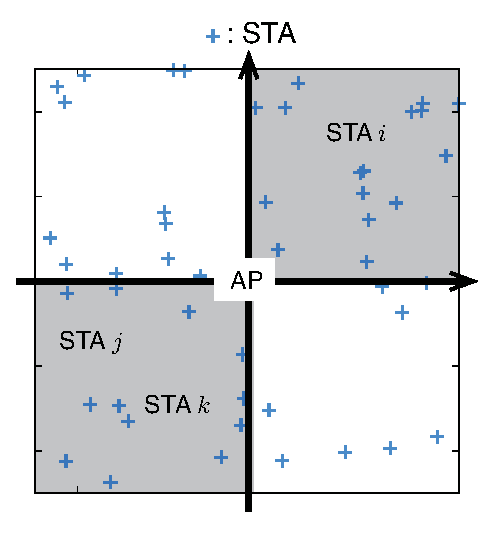
\epsfig{file=fig/time.eps, scale=0.8}
				\caption{位置によるSTAのグループ分け}
				\label{fig:time_image}
			\end{figure}
			本節では,最適化問題を解くための計算時間を削減する手法について検討する.
			第\ref{sec:opt}節で述べたように,APは最適化問題を定期的に解き確率$\pijk$を更新する.
			確率$\pijk$は,STAの参加離脱,移動による$\rijk$の変化,$d^{(j)}$,$d^{(k)}$の更新など状態の変化に追従するよう更新する必要があるため,
			数百ミリ秒単位で最適化問題を解く必要がある.
			提案方式の最適化問題は線形最適化問題であるが,Karmarkarの内点法~\cite{karmarkar}を用いる場合,
			計算量は変数の数$n$に対して$O(n^{3.5})$であり,指数的に増加する.
			変数の数は送受信STAの組み合わせの数$|{\mthc}|$であり,STA台数を$N$台,OFDMAの多重数を$M$とすると,
			最大で$(N+1)N^M-1$となる.
			そのため,$N$が大きくなると計算量が爆発的に大きくなる.
			\par
			そこで,本論文では計算時間削減の初期検討として,選択可能なSTA組を制限する手法を検討する.
			ある送受信STA組におけるスループットはユーザ間干渉が大きいほど減少する傾向にある.
			また,ユーザ間干渉の大きさはSTAの地理的位置に依存し,受信STAと送信STAとの距離が遠いほど干渉が小さくなる傾向にある.
			そこで,STAを位置によってグループ分けし特定のSTA組に限定することで組み合わせの数を削減する.
			\par
			STAの組み合わせをユーザ間干渉が小さくなる可能性が高い組み合わせのみに限定するため,
			下り通信を行うSTA $i$と上り通信を行う2台のSTA $j$,$k$がAPを中心として対角の位置に存在する組み合わせのみを最適化の対象とする.
			図\ref{fig:time_image}のようにAPを中心とした直交座標を設定し,それぞれのSTAがどの象限に位置するかによって4つのグループに分ける.
			そして,組み合わせの集合$\mthc$には,OFDMAとUFD通信を組み合わせる場合はSTA $i$と2台のSTA $j$,$k$は対角の象限,STA $j$と$k$は同じ象限に存在するような組み合わせ,UFD通信の場合はSTA$i$と$j$は対角の象限に存在する組み合わせのみを含める.

\section{シミュレーション評価}
	\subsection{シミュレーションモデル}
		本節では,各提案方式に関するシミュレーションのモデルと条件に関して述べる.
		\subsubsection{フレーム時間長最適化}
			本項では,フレーム時間長最適化に関するシミュレーションのモデルについて述べる.
			本シミュレーションにおいては,APとSTAが1台ずつ存在し,それらは完全な自己干渉除去技術をもった全二重通信対応端末であるとする.
			いずれもバッファに送信すべきデータフレームが存在する限り必ず全二重通信を行うものとする.
			また,RTSフレームの同時送信による衝突を除いては,データフレームの送受信は成功するものとする.
			AP,STAのMAC層に到着するデータフレームはポアソン分布に従い,その到着率をそれぞれ$\lambda_{\rm{AP}}$\,frames/s,
			$\lambda_{\rm{STA}}$\,frames/sとする.
			さらに,実際の無線LAN利用時におけるトラヒックは下り通信が支配的であることから,
			$\lambda_{\rm{AP}}=10^{5}$として固定する~\cite{traffic}.
			APとSTAに到着するIPパケット長は図\ref{fig:traffic}に示す分布に従う.
			これは,実際に\cite{traffic}によって測定されたIPパケット長の分布を簡単化したものである.
			データフレームの送信にはA-MSDUのみを用いる.
			伝送速度は65\,Mbit/sとし,APとSTAのバッファサイズは200\,kBとする.
			MAC層に関する詳細はIEEE 802.11n~\cite{stdn}に従う.
			シミュレーション時間は5分である.
			\par
			本シミュレーションでは3つの方式の比較を行う.
			1つ目は比較方式として最適化を第一段階までとしたものであり,2つ目は第二段階で用いるデータフレーム数の上限を$n=1$とした提案方式であり,
			3つ目は上限を設けない提案方式である.
			これら3つの方式に対して,平均遅延時間,平均無駄時間,システムスループットの結果を示す.
			遅延時間とはあるデータフレームが送信バッファに到着してから送信されるまでの時間である.

			\begin{figure}[t]
				\begin{center}
					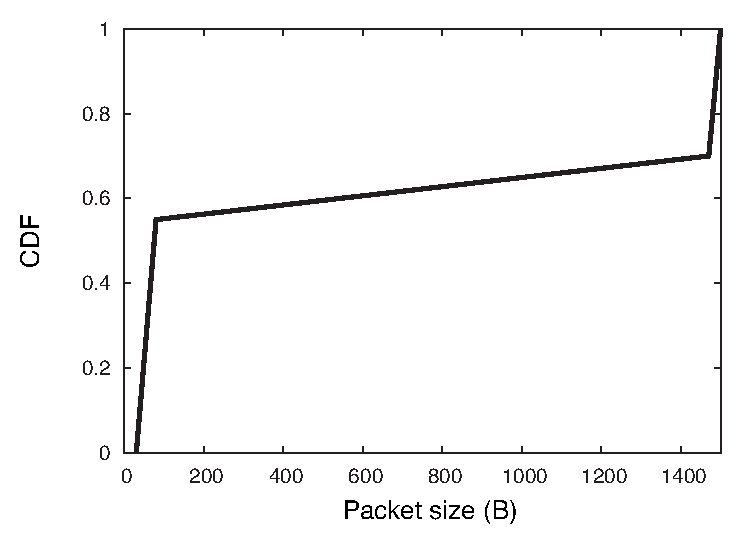
\includegraphics[width=0.7\textwidth]{graph/traffic.eps}
					\caption{Packet size distribution used in simulations.}
					\label{fig:traffic}
				\end{center}
			\end{figure}

		\subsubsection{UFD通信におけるSTA選択}
			本項ではUFD通信におけるSTA選択手法に関するシミュレーションのモデルについて述べる.
			図\ref{fig:pos}のように,1台のAPが$L=100$\,m四方の領域の中心に設置され,その周りに$N=50$台のSTAがランダムに配置されているとする.
			MACプロトコルは~\cite{promac}に従い,従来の目的関数,及び,$\etau$設定法を用いたものと提案の目的関数,及び,$\etau$設定法を用いたものを比較する.
			上下通信ともに飽和トラヒックの場合を取り扱う.

			\begin{figure}[t]
				\begin{center}
					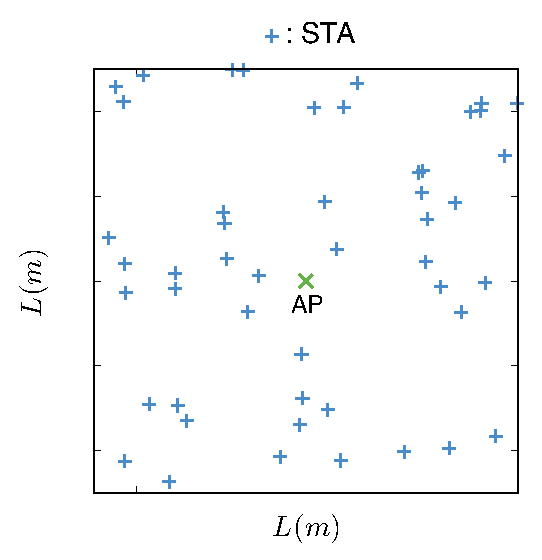
\includegraphics[width=0.7\textwidth]{fig/pos.eps}
					\caption{Packet size distribution used in simulations.}
					\label{fig:pos}
				\end{center}
			\end{figure}

			\begin{table}[t]
				\centering
				\caption{UFD通信におけるSTA選択手法に関するシミュレーションの諸元}
				\label{tab:param}
				\begin{tabular}{cc} \hline
					領域の大きさ $L$ & 100\,m \\
					伝送速度 & シャノン容量 \\
					送信電力 & 15\,dBm \\
					雑音指数 & 10\,dB \\
					周波数帯 & 2.4\,GHz \\
					帯域幅 & 20\,MHz \\
					伝搬損失 & $30\log D + 40$\\
					&($D$: 送受信点間距離)\\
					自己干渉除去 & 110\,dB \\
					シミュレーション時間 & 10\,s \\\hline
				\end{tabular}
			\end{table}

		\subsubsection{上りOFDMAによるUFD通信通信の遅延時間削減}
			本項では上りOFDMAによるUFD通信通信の遅延時間削減に関するシミュレーションのモデルについて述べる.
			全節と同様,図\ref{fig:pos}のように,1台のAPが$L=100$\,m四方の領域の中心に設置され,その周りに$N=50$台のSTAがランダムに配置されているとする.
			MACプロトコルは~\cite{promac}に従う.
			シミュレーションは最適化問題はMATLABにより計算し,そのほかの部分はC言語で作成したシミュレータによって行う.
			半二重通信のみを用いる場合,半二重通信とUFD通信を併用する従来方式~\cite{promac_fair}と,
			半二重通信,UFD通信,上りOFDMA,UFD通信と上りOFDMAの組み合わせの4方式を用いる提案方式を比較する.
			OFDMAによる多重化は簡単のため二多重までとし,チャネル幅は二等分するものとする.
			式\eqref{eq:etad}における$\eta_{\rm d}^{(i)}$には各STA共通の$1/[(N+1)N]$を,
			式\eqref{eq:etau}における$\eta_{\rm u}^{(l)}$には各STA共通の$1/(N+1)$を設定している.
			伝送速度はIEEE 802.11aに従う.
			上下通信ともに飽和トラヒックであり,APには1500\,Bの,STAには64\,Bのデータフレームが発生しているものとする.
			これは,トラヒックの多くがTCP-ACKを中心とする64\,B以下のフレームと1500\,Bのフレームによって占められるからである~\cite{traffic}.
	\subsection{フレーム時間長最適化}
		\subsubsection{A-MSDUの最大長に対する結果}
			まず,A-MSDUの最大長を2000\,Bから7935\,bytesまで変化させた場合における結果を示す.
			この結果においてはSTAのフレーム到着率は$\lambda_{\rm STA}=10^5$とする.
			図\ref{fig:dly_max}にA-MSDUの最大長に対する平均遅延を示す.
			比較方式に比べて,$n=1$とした提案方式は遅延時間を13\%,制限を設けない提案方式は遅延時間を49\%削減している.
			これは,制限を設けない提案方式は最適化の第二段階において小さなデータフレームをたくさん用いることができ,
			その結果,小さなデータフレームの遅延時間が大きく削減されるためである.
			\par
			次に,図\ref{fig:wst_max}にA-MSDUの最大長に対する平均無駄時間を示す.
			比較方式に比べて,$n=1$とした提案方式ではむだ時間を97\%削減しており,
			さらに,制限を設けない提案方式では,$n=1$とした提案方式に比べて無駄時間を96\%削減している.
			\par
			図\ref{fig:thr_max}にA-MSDUの最大長に対するシステムスループットを示す.
			A-MSDUの最大長が2000\,Bの場合においては,$n=1$とした提案方式は比較方式に対してシステムスループットを15\%増加させている.
			一方で,制限を設けない提案方式は,$n=1$とした提案方式と比較してシステムスループットをほとんど改善しない.
			これは,ほとんどの送信機会において$n=1$とした提案方式が無駄時間をIEEE 802.11a規格の無線LANで用いらているOFDMのシンボル長である$4\,\mu$以下にまで削減できているためである.
			制限を設けない提案方式は$n=1$とした提案方式と比較してプライマリセンダとセカンダリセンダのフレーム時間長が完全に一致する割合が増えているものの,
			その差は僅かであるためシステムスループットの改善幅は小さい.
			\par
			以上の結果から,本シミュレーション条件においては最適化に必要な時間を考慮すると,第二段階で用いるデータフレーム数の上限$n$は1で良いと言える.

		\subsubsection{vs. Frame Arrival Rate of STA}
			次に,STAのフレーム到着率$\lambda_{\rm STA}$を$10^2$から$10^5$に変化させた場合の結果について述べる.
			本シミュレーションにおいてはA-MSDUの最大長は7935\,Bとする.
			図\ref{fig:dly_lmd}にSTAのフレーム到着率に対する平均遅延時間を示す.
			比較方式に対して,$n=1$とした提案方式は遅延時間を33\%,制限を設けない提案方式は遅延時間を45\%削減している.
			\par
			図\ref{fig:wst_lmd}にSTAのフレーム到着率に対する平均無駄時間を示す.
			$n=1$とした提案方式は,STAのフレーム到着率が$\lambda_{\rm STA}\geq 2 \times 10^{4}$の場合において,
			無駄時間を比較方式に対して97\%削減できている.
		 	さらに,制限を設けない提案方式は,$n=1$とした提案方式に対して無駄時間を96\%削減している.
			\par
			図\ref{fig:thr_lmd}にSTAのフレーム到着率に対するシステムスループットを示す.
			提案方式は$n=1$とした場合と制限を設けない場合とで同程度の値を示し,
			比較方式に対しては$\lambda_{\rm STA} \geq 2 \times 10^{4}$においてシステムスループットを4.7\%改善している.
			\par
			以上の結果から,STAのフレーム到着率が大きいときには提案方式による性能の改善が見られる一方,
			STAのフレーム到着率が小さいときには提案方式による性能の改善がわずかであることがわかった.
			STAのオファードロードが飽和している場合はSTAのバッファにはたくさんのデータフレームが存在し,
			提案方式によってフレーム時間長を最適化する際にアグリゲーションに用いるデータフレームの選択肢が多いことと同義であり,
			その結果,提案方式による性能改善効果が得られる.
			一方,STAのオファードロードが非飽和である場合は,STAのバッファにデータフレームが溜まりにくく,
			フレーム時間長を最適化する際のアグリゲーションの組み合わせの数が少なくなるため,
			飽和時と比べて提案方式による性能改善効果が得られにくいことが原因である.

			\begin{figure}[t]
				\begin{center}
					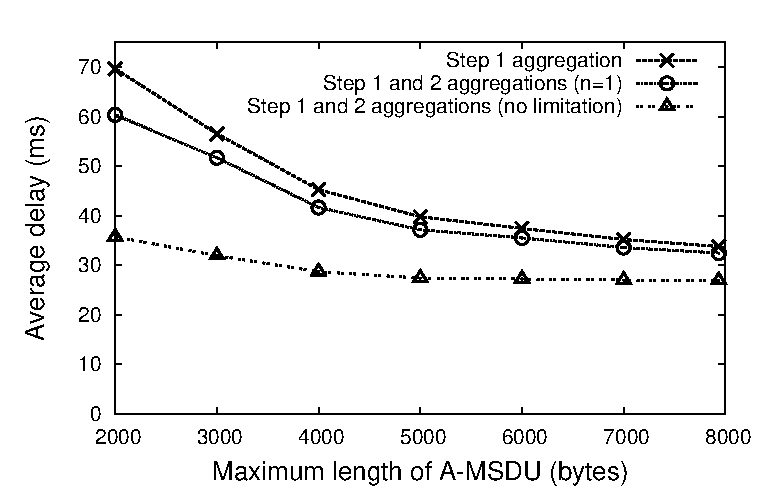
\includegraphics[width=0.8\textwidth]{graph/dly_max.eps}
					\caption{Average delay vs. maximum length of A-MSDU when $\lambda_{\rm AP}$ and $\lambda_{\rm STA}$ are $10^{5}$.}
					\label{fig:dly_max}
				\end{center}
			\end{figure}
			\begin{figure}[t]
				\begin{center}
					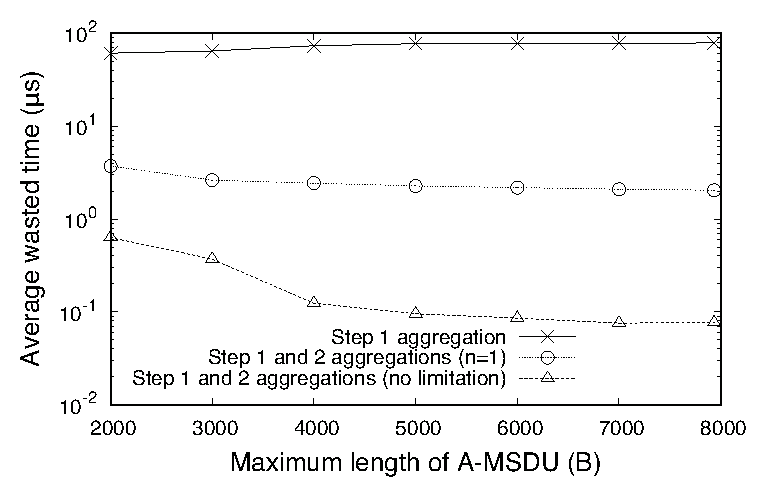
\includegraphics[width=0.8\textwidth]{graph/wst_max.eps}
					\caption{Average wasted time vs. maximum length of A-MSDU when $\lambda_{\rm AP}$ and $\lambda_{\rm STA}$ are $10^{5}$.}
					\label{fig:wst_max}
				\end{center}
			\end{figure}

			\begin{figure}[t]
				\begin{center}
					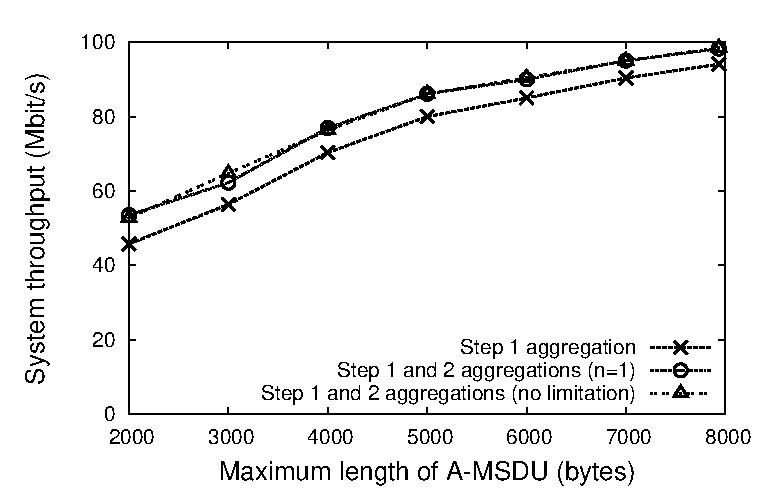
\includegraphics[width=0.8\textwidth]{graph/thr_max.eps}
					\caption{Throughput vs. maximum length of A-MSDU when $\lambda_{\rm AP}$ and $\lambda_{\rm STA}$ are $10^{5}$.}
					\label{fig:thr_max}
				\end{center}
			\end{figure}
			\begin{figure}[t]
				\begin{center}
					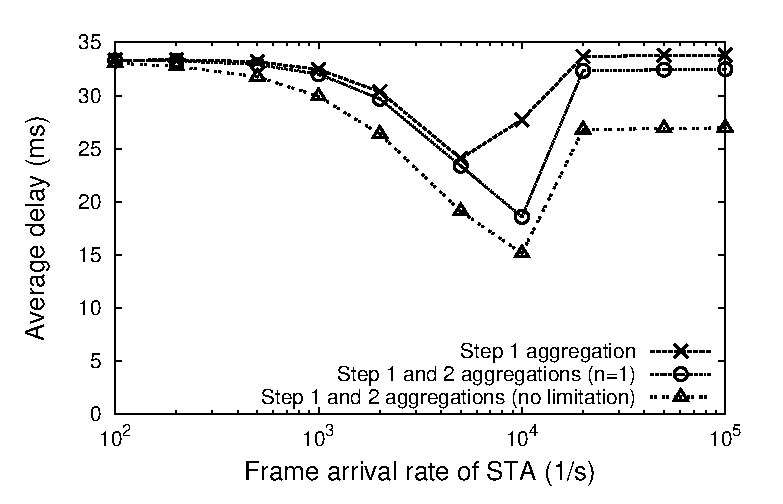
\includegraphics[width=0.8\textwidth]{graph/dly_lmd.eps}
					\caption{Average delay vs. frame arrival rate of STA when maximum length of A-MSDU is 7935\,bytes.}
					\label{fig:dly_lmd}
				\end{center}
			\end{figure}
			\begin{figure}[t]
				\begin{center}
					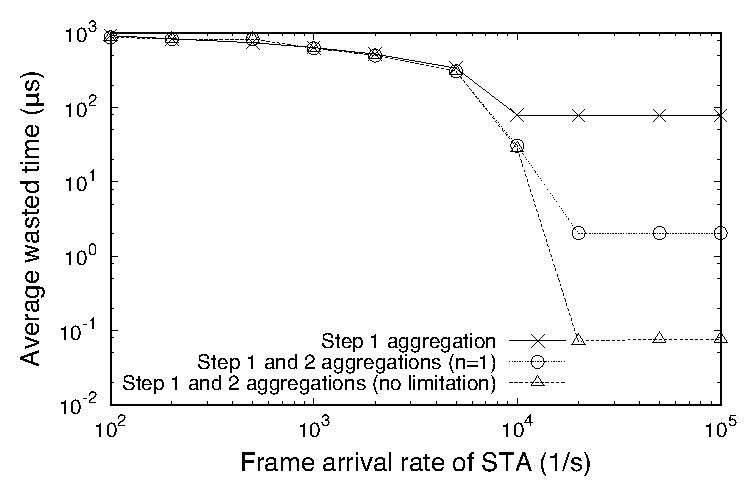
\includegraphics[width=0.8\textwidth]{graph/wst_lmd.eps}
					\caption{Average wasted time vs. frame arrival rate of STA when maximum length of A-MSDU is 7935\,bytes.}
					\label{fig:wst_lmd}
				\end{center}
			\end{figure}
			\begin{figure}[t]
				\begin{center}
					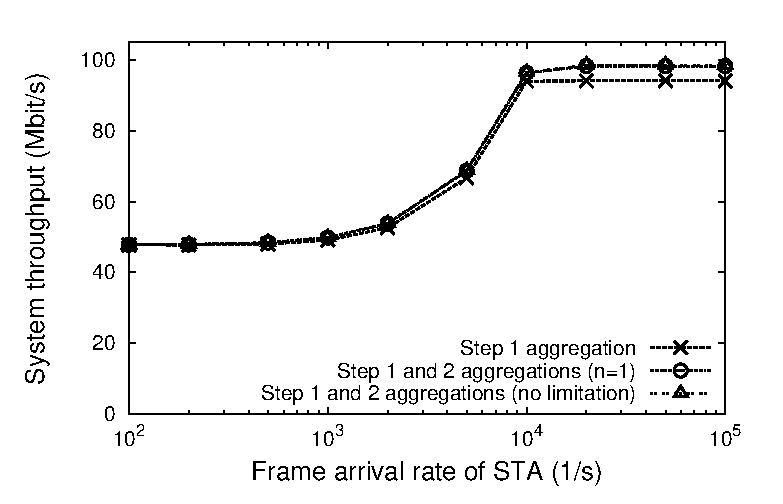
\includegraphics[width=0.8\textwidth]{graph/thr_lmd.eps}
					\caption{Troughput vs. frame arrival rate of STA when maximum length of A-MSDU is 7935\,bytes.}
					\label{fig:thr_lmd}
				\end{center}
			\end{figure}
	\subsection{UFD通信におけるSTA選択}
		\subsubsection{公平性の改善}
			図\ref{fig:fair}にSTA台数を$N=50$とした場合の各STAの全シミュレーション時間内での上り通信送信回数を示す.
			図\ref{fig:numtx}と比較して,一部のSTAが極端に選ばれやすいという現象が改善されていることがわかる.
			図\ref{fig:thr_fair}にシステムスループットとSTA間の公平性を示す.
			ただし,結果は10種類の異なるSTA配置によるシミュレーション結果の平均値であり,
			公平性はJain's fairness index~\cite{jain}における各STAのスループットを送信回数に置き換えたもので評価した.
			また,$\alpha=0$は従来方式の結果とする.
			提案方式は$\alpha$を適切に設定することで,従来方式と比較してSTA間の送信機会に関する公平性を大きく改善できることを示した.
			更に,提案方式において重み係数$\alpha$を変化させることで,公平性の改善とシステムスループット低下のトレードオフを調整可能であることを示した.
			また,本シミュレーションでは$\alpha\leq0.4$のときに従来方式と比較してシステムスループットの低下が小さく,公平性が高くなっている.
			\par
			次に,シミュレーション条件の違いによる重み係数$\alpha$の影響の差について検討する.
			STA台数が結果に与える影響を確認するため,図\ref{fig:chgnum}にSTA台数を$N=30$とした場合の結果を示す.
			ただし,結果は10種類の異なるSTA配置によるシミュレーション結果の平均値である.
			本シミュレーションでは,$\alpha=0.3$において公平性の改善が飽和しているにも関わらず,
			$0.3<\alpha$ではシステムスループットが従来方式と比較して大きく低下しているため,$0.3<\alpha$とする必要はない.
			続いて,図\ref{fig:chgtopology}にあるSTA配置におけるシステムスループットとSTA間の公平性を示す.
			本シミュレーションでは,$\alpha\leq0.4$においてはシステムスループットを大きく低下させることなく公平性を改善できている.
			一方,$0.5\leq\alpha$ではシステムスループットが大きく低下している.
			以上,二つの結果から従来方式と比較してシステムスループットを大きく低下させることなく公平性を改善できているのは
			概ね$0.1\leq\alpha\leq0.3$の範囲である.

			\begin{figure}[t]
				\centering
				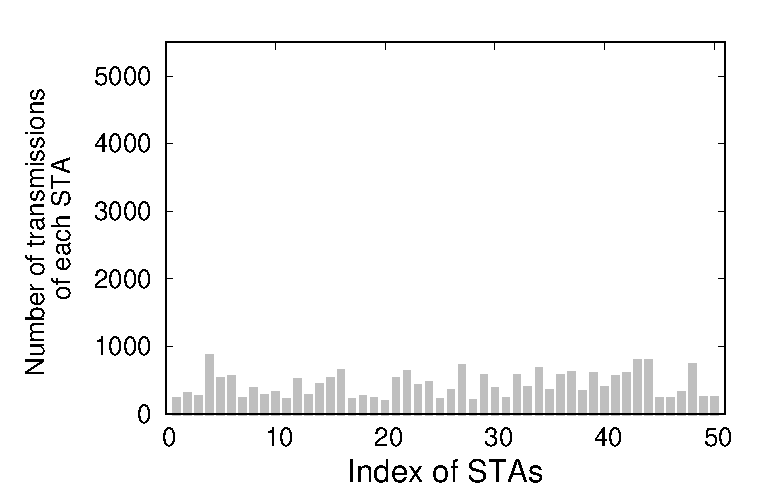
\epsfig{file=graph/numtxfair.eps, scale=0.8}
				\caption{提案方式によるSTAの上り通信送信回数の分布}
				\label{fig:fair}
			\end{figure}

			\begin{figure}[t]
				\centering
				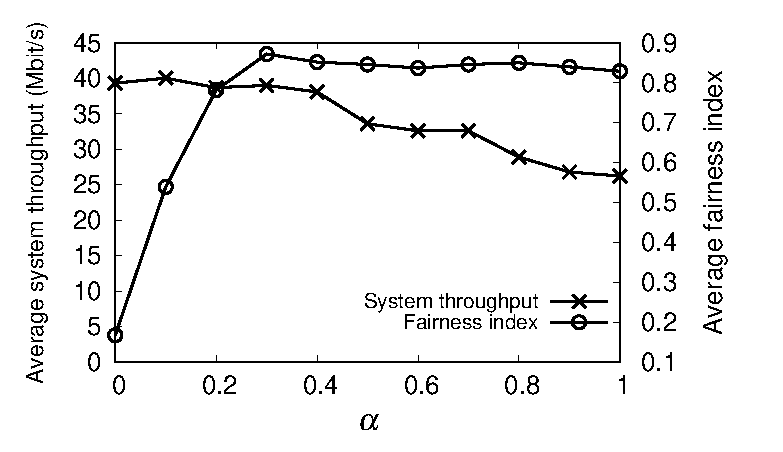
\epsfig{file=graph/thr_fair.eps, scale=0.8}
				\caption{重み係数$\alpha$に対するシステムスループットとfairness index}
				\label{fig:thr_fair}
			\end{figure}

			\begin{figure}[t]
				\centering
				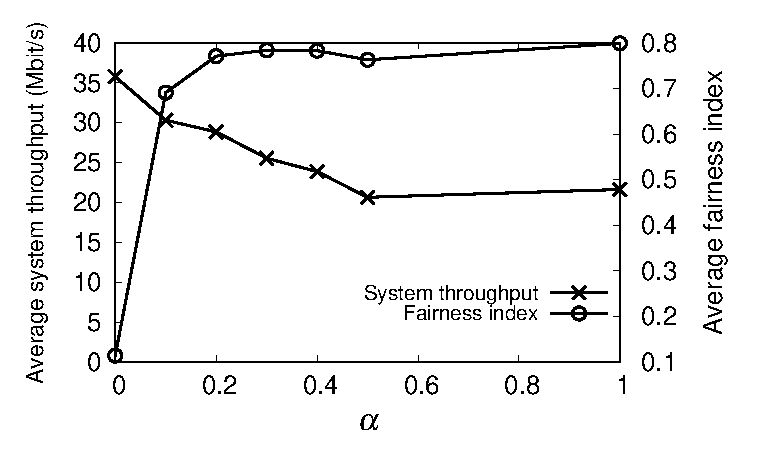
\epsfig{file=graph/chgnum.eps, scale=0.8}
				\caption{STA台数を$N=30$に変更した場合の重み係数$\alpha$に対するシステムスループットとfairness index}
				\label{fig:chgnum}

				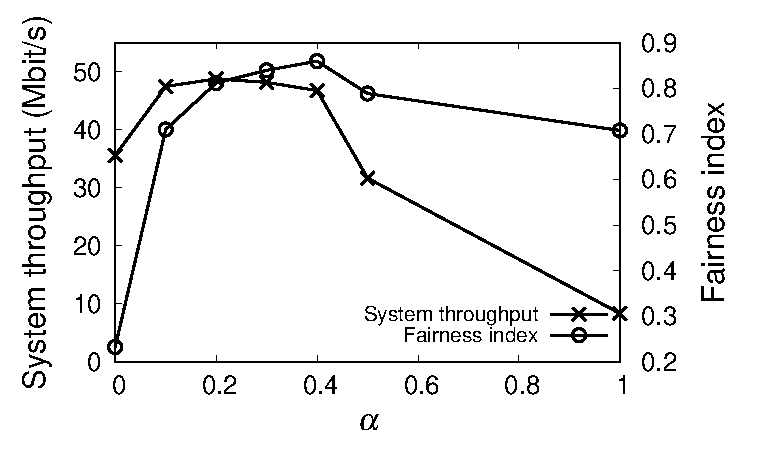
\epsfig{file=graph/chgtopology.eps, scale=0.8}
				\caption{あるSTA配置における重み係数$\alpha$に対するシステムスループットとfariness index}
				\label{fig:chgtopology}
			\end{figure}

		\subsubsection{低遅延を要求するSTAのQoSの向上}
			次に,低遅延を要求するSTAのQoS向上について評価を行う.
			全STA台数は$N=50$とし,低遅延を要求するSTAを${\mathcal D}=\{46,\ 47,\ 48,\ 49,\ 50\}$とした.
			式\eqref{eq:etadbar}における$x_j$は,
			低遅延を要求しないSTAすべてで共通の値$x_j=x,\ \forall j\in {\overline {\mathcal D}}$とし,
			式\eqref{eq:etad}における$x_j'$も低遅延を要求するSTAすべてで共通の値$x_j'=x|{\overline {\mathcal D}}|/|{\mathcal D}|,\ \forall j \in {\mathcal D}$とした.ただし,$|{\overline {\mathcal D}}|$は低遅延を要求しないSTAの台数,
			$|{\mathcal D}|$は低遅延を要求するSTAの台数を表す.
			また,$\alpha=0.3$とし,いずれもある1種のSTA配置についての結果である.
			\par
			まず,図\ref{fig:chnx}に$x$の値に対する低遅延を要求する5台のSTAの平均送信間隔を示す.
			$x=0$の時が従来方式の場合の結果である.
			従来方式と比較して,$x$を大きくするほど低遅延を要求する5台のSTAの平均送信間隔が小さくなっている.
			この結果から,アプリーケーションサービスが要求する遅延時間に応じて送信間隔を調整可能であることがわかる.
			\par
			次に$x=0.005$としたときのすべてのSTAの平均送信間隔について評価する.
			図\ref{fig:inter}\subref{fig:interfair}に公平性のみを考慮した場合について,
			図\ref{fig:inter}\subref{fig:intereta}に提案方式を用いた場合について各STAの平均送信間隔を示す.
			公平性のみを考慮した場合は全STA間の送信機会の公平性が高いことから,
			送信間隔のばらつきが少ないが,低遅延を要求するSTA 46から50の送信間隔も平均43\,msと長い.
			一方,提案手法を用いた場合,送信間隔を15\,msと1/3程度まで削減することができた.
			しかし,低遅延を要求しないSTAの送信間隔のばらつきが大きくなった.
			この問題の解決は今後の課題とする.

			\begin{figure}[t]
				\centering
				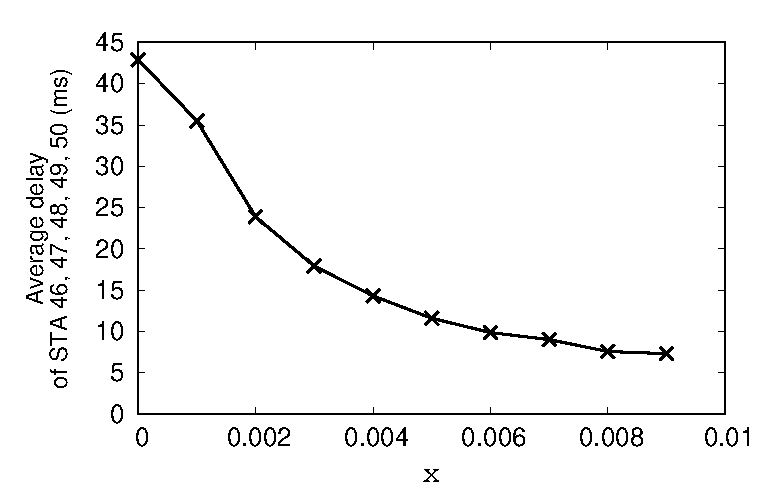
\epsfig{file=graph/chnx.eps, scale=0.8}
				\caption{$x$に対する低遅延を要求するSTAの平均送信間隔}
				\label{fig:chnx}
			\end{figure}

			\begin{figure}[t]
				\centering
				\subfloat[公平性の改善のみを行った場合のSTAの平均送信間隔]{
					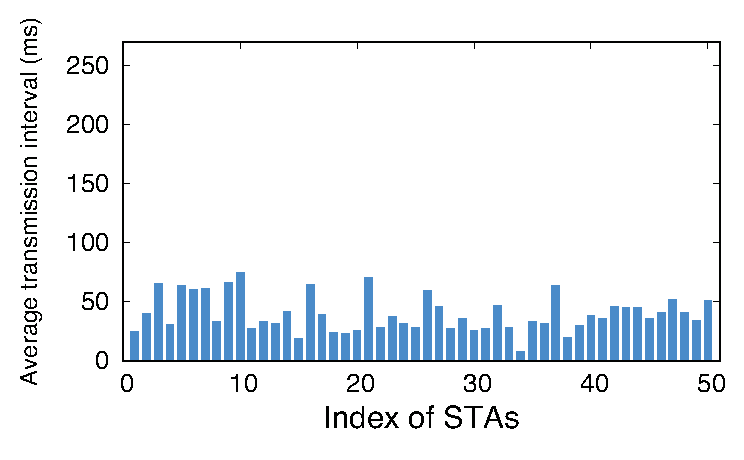
\epsfig{file=graph/interfair.eps, scale=0.8}
					\label{fig:interfair}
				}
				\\
				\subfloat[低遅延を要求するSTAの送信機会を増加させた場合のSTAの平均送信間隔]{
					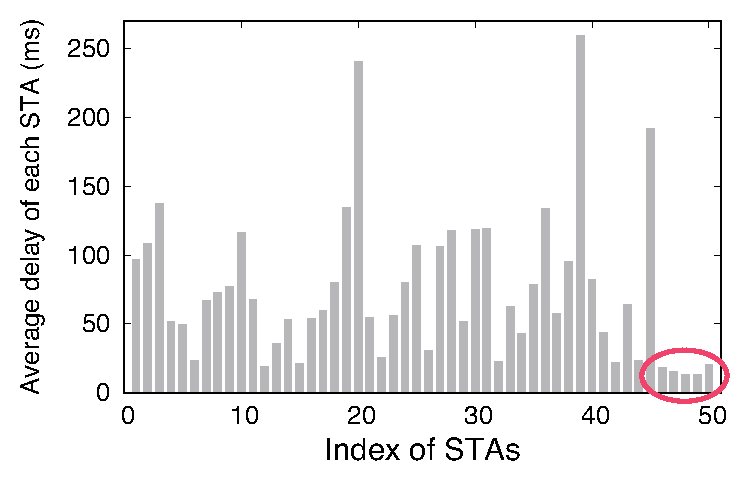
\epsfig{file=graph/intereta.eps, scale=0.8}
					\label{fig:intereta}
				}
				\caption{STAの平均送信間隔の比較}
				\label{fig:inter}
			\end{figure}

	\subsection{上りOFDMAによるUFD通信通信の遅延時間削減}
		本章では提案手法の有効性をシミュレーションによって評価する.
		シミュレーションは最適化問題はMATLABにより計算し,そのほかの部分はC言語で作成したシミュレータによって行う.
		半二重通信のみを用いる場合,半二重通信とUFD通信を併用する従来方式~\cite{promac_fair}と,
		半二重通信,UFD通信,上りOFDMA,UFD通信と上りOFDMAの組み合わせの4方式を用いる提案方式を比較する.
		OFDMAによる多重化は簡単のため二多重までとし,チャネル幅は二等分するものとする.
		図\ref{fig:model}のように,1台のAPが $L=$100\,m四方の領域の中心に設置され,その周りに$N=50$台のSTAがランダムに配置されているとする.
		式\eqref{eq:etad}における$\eta_{\rm d}^{(i)}$には各STA共通の$1/[(N+1)N]$を,
		式\eqref{eq:etau}における$\eta_{\rm u}^{(l)}$には各STA共通の$1/(N+1)$を設定している.
		伝送速度はIEEE 802.11aに従う.
		上下通信ともに飽和トラヒックであり,APには1500\,Bの,STAには64\,Bのデータフレームが発生しているものとする.
		これは,トラヒックの多くがTCP-ACKを中心とする64\,B以下のフレームと1500\,Bのフレームによって占められるからである~\cite{traffic}.

		\begin{figure}[t]
			\centering
			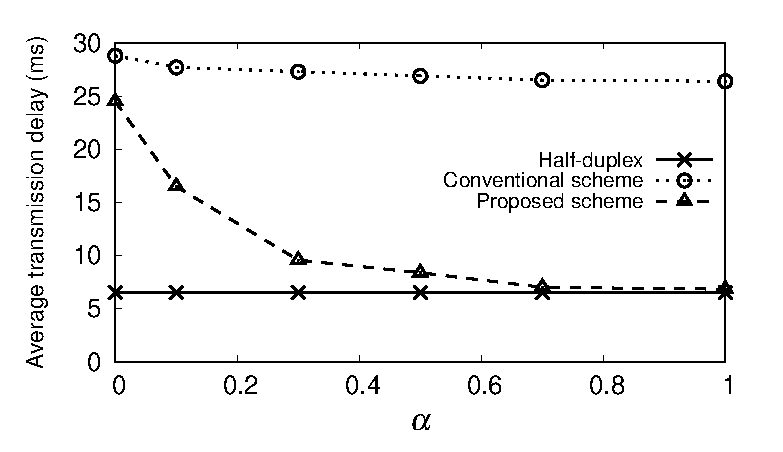
\epsfig{file=graph/delay.eps, scale=0.8}
			\caption{上り通信の平均遅延時間}
			\label{fig:delay}
		\end{figure}
		\begin{figure}[t]
			\centering
			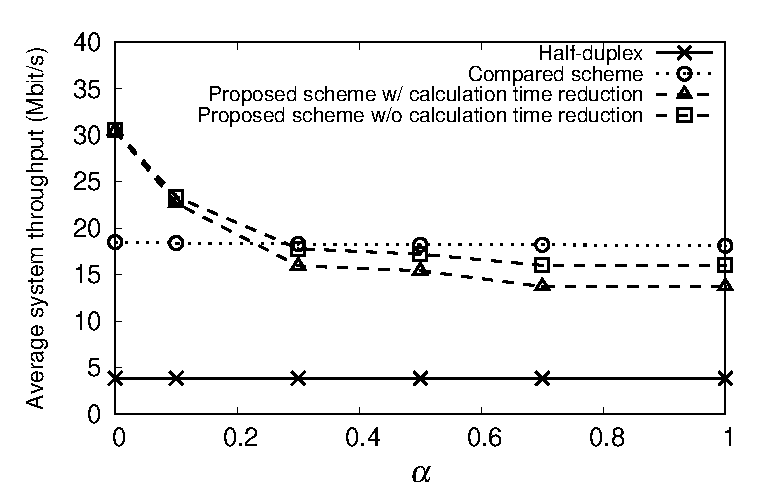
\epsfig{file=graph/thr.eps, scale=0.8}
			\caption{システムスループット}
			\label{fig:thr}
		\end{figure}
		\begin{figure}[t]
			\centering
			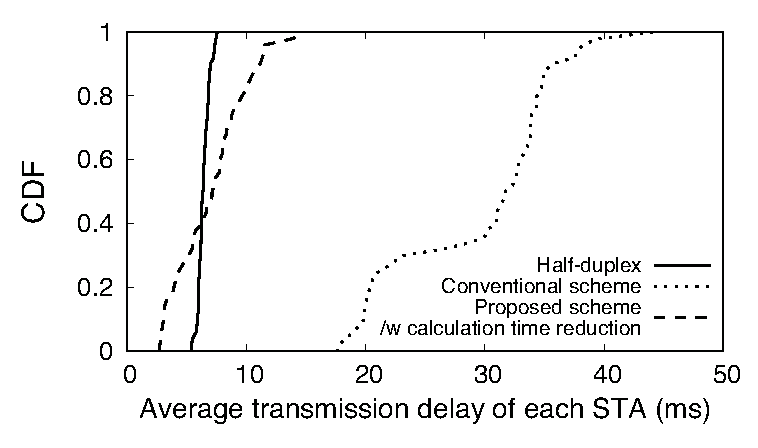
\epsfig{file=graph/cdf.eps, scale=0.8}
			\caption{ある試行における各STAの平均遅延時間のCDF}
			\label{fig:cdf}
		\end{figure}

		\par
		図\ref{fig:delay},\ref{fig:thr}にSTAの平均遅延時間とシステムスループットを示す.
		半二重通信とUFD通信を用いる従来方式の遅延時間は半二重通信と比べ20\,ms以上大きい.
		一方,提案方式はパラメータ$\alpha$を大きくすることで遅延時間を半二重通信と同等の値まで削減できている.
		しかし,$\alpha$が大きくなるにつれて,システムスループットが低下している.
		これは,最適化問題の目的関数において$d^{(j)},\ d^{(k)}$の項の影響が大きくなり,スループットの低下による利得の減少より遅延時間削減による利得向上が上回るためである.
		提案方式はシステムスループットは低下したものの,半二重通信に対しては3倍程度の値を維持しつつ,
		遅延時間を半二重通信と同等まで削減することができた.
		\par
		STA間の公平性を示すため,図\ref{fig:cdf}に各STA毎の平均遅延時間のCDF(Cumulative distribution functioin)を示す.
		半二重通信では全STAが平等に送信機会を獲得するため,STA間の遅延時間のばらつきは非常に小さい.
		提案方式は半二重通信には及ばないものの,従来方式と比べて大幅にばらつきが小さくなっており,
		遅延時間に対する公平性が高いことを示している,

		\begin{table}[t]
			\centering
			\caption{最適化問題を1回解くために必要な平均時間}
			\label{tab:time}
			\begin{tabular}{cc}
			 計算時間削減なし & 計算時間削減あり\\ \hline
			 803\,ms & 226\,ms \\\hline
			\end{tabular}
		\end{table}
%		\begin{figure}[t]
%			\centering
%			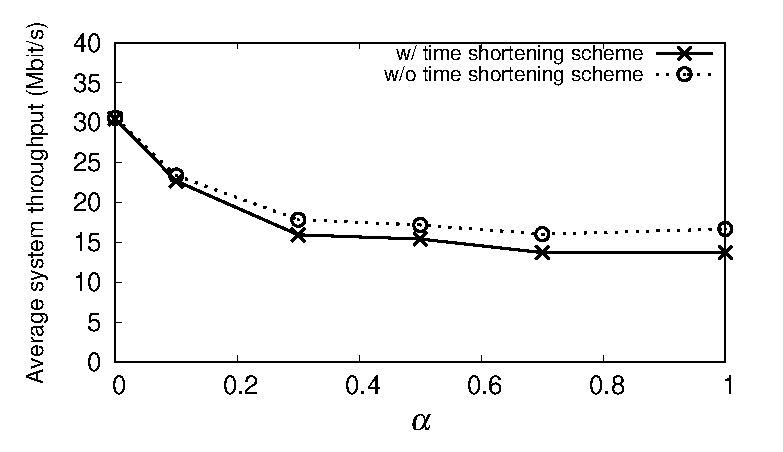
\epsfig{file=graph/thr_time.eps, scale=0.6}
%			\caption{システムスループットへの計算時間削減手法の影響}
%			\label{fig:thr_time}
%		\end{figure}

		\par
		次に計算時間について評価する.
		表\ref{tab:time}に第\ref{sec:time}節で述べた計算時間削減手法を用いた場合と用いない場合について,
		$\alpha=1$における最適化問題を一回解くために必要な平均時間を示す.
		計算時間を72\%削減できている一方,送受信STAの組み合わせを制限するため,利得の高い組み合わせまで除外されることがありシステムスループットが低下する.
		図\ref{fig:thr}より計算量削減手法を用いた場合でもシステムスループットの低下は最大18\%となった.
		簡易な方式ながら,システムスループットを大幅に低下させることなく,計算時間を削減することができた.

\section{まとめ}

\acknowledgments				% 謝辞
	本研究を行うにあたり,多くの方々にお世話になりました.
	ここに深く感謝の意を表します.
 守倉正博教授には本研究の機会を与えて頂き,また貴重な御助言を頂きましたことを深く感謝致します.
 西尾理志助教には,本研究を行うにあたり,熱心な御指導をして頂き,多大なご協力をして頂きましたことを深く感謝致します.
 山本高至准教授には本研究を進めるにあたり,適切な御助言を頂きまして深く感謝致します.
 株式会社東芝の鍋谷寿久様,青木亜秀様には,本研究を進めるにあたり数多くの御指導,御支援を頂きましたことを深く感謝致します.
 本研究にあたって,あらゆる面で数々の貴重な御意見,御協力を頂いた守倉研究室の皆様方に心より感謝致します.

\bibliographystyle{sieicej}			% 文献スタイルの指定
\bibliography{main2.bib}				% 参考文献の出力
\end{document}
